%  LaTeX support: latex@mdpi.com 
%  For support, please attach all files needed for compiling as well as the log file, and specify your operating system, LaTeX version, and LaTeX editor.

%=================================================================
\documentclass[symmetry,article,submit,pdftex,moreauthors]{Definitions/mdpi} 
%\documentclass[preprints,article,submit,pdftex,moreauthors]{Definitions/mdpi} 
% For posting an early version of this manuscript as a preprint, you may use "preprints" as the journal. Changing "submit" to "accept" before posting will remove line numbers.

% Below journals will use APA reference format:
% admsci, aieduc, behavsci, businesses, econometrics, economies, education, ejihpe, famsci, games, humans, ijcs, ijfs, journalmedia, jrfm, jsam, languages, peacestud, psycholint, publications, tourismhosp, youth

% Below journals will use Chicago reference format:
% arts, genealogy, histories, humanities, jintelligence, laws, literature, religions, risks, socsci

%--------------
% Class Options:
%--------------
%-------
% journal
%-------
% Choose between the following MDPI journals:
% accountaudit, acoustics, actuators, addictions, adhesives, admsci, adolescents, aerobiology, aerospace, agriculture, agriengineering, agrochemicals, agronomy, ai, aichem, aieduc, aieng, aimater, aimed, aipa, air, aisens, algorithms, allergies, alloys, amh, analog, analytica, analytics, anatomia, anesthres, animals, antibiotics, antibodies, antioxidants, applbiosci, appliedchem, appliedmath, appliedphys, applmech, applmicrobiol, applnano, applsci, aquacj, architecture, arm, arthropoda, arts, asc, asi, astronautics, astronomy, atmosphere, atoms, audiolres, automation, axioms, bacteria, batteries, bdcc, behavsci, beverages, biochem, bioengineering, biologics, biology, biomass, biomechanics, biomed, biomedicines, biomedinformatics, biomimetics, biomolecules, biophysica, bioresourbioprod, biosensors, biosphere, biotech, birds, blockchains, bloods, blsf, brainsci, breath, buildings, businesses, cancers, carbon, cardiogenetics, cardiovascmed, catalysts, cells, ceramics, challenges, chemengineering, chemistry, chemosensors, chemproc, children, chips, cimb, civileng, cleantechnol, climate, clinbioenerg, clinpract, clockssleep, cmd, cmtr, coasts, coatings, colloids, colorants, commodities, complexities, complications, compounds, computation, computers, condensedmatter, conservation, constrmater, cosmetics, covid, crops, cryo, cryptography, crystals, csmf, ctn, culture, curroncol, cyber, dairy, data, ddc, dentistry, dermato, dermatopathology, designs, devices, dhi, diabetology, diagnostics, dietetics, digital, disabilities, diseases, diversity, dna, drones, dynamics, earth, ebj, ecm, ecologies, econometrics, economies, edm, education, eesp, ejihpe, electricity, electrochem, electronicmat, electronics, encyclopedia, endocrines, energies, eng, engproc, entomology, entropy, environments, environremediat, epidemiologia, epigenomes, esa, est, famsci, fermentation, fibers, fintech, fire, fishes, fluids, foods, forecasting, forensicsci, forests, fossstud, foundations, fractalfract, fuels, future, futureinternet, futurepharmacol, futurephys, futuretransp, galaxies, games, gases, gastroent, gastrointestdisord, gastronomy, gels, genealogy, genes, geographies, geohazards, geomatics, geometry, geosciences, geotechnics, geriatrics, germs, glacies, grasses, green, greenhealth, gucdd, hardware, hazardousmatters, healthcare, hearts, hemato, hematolrep, hep, heritage, higheredu, highthroughput, histories, horticulturae, hospitals, humanities, humans, hydrobiology, hydrogen, hydrology, hydropower, hygiene, idr, iic, ijcs, ijem, ijerph, ijfs, ijgi, ijmd, ijms, ijns, ijom, ijpb, ijt, ijtm, ijtpp, ime, immuno, informatics, information, infrastructures, inorganics, insects, instruments, inventions, iot, j, jaestheticmed, jal, jcdd, jcm, jcp, jcrm, jcs, jcto, jdad, jdb, jdream, jemr, jeta, jfb, jfmk, jgbg, jgg, jimaging, jintelligence, jlpea, jmahp, jmmp, jmms, jmp, jmse, jne, jnt, jof, joi, joitmc, joma, jop, joptm, jor, journalmedia, jox, jpbi, jphytomed, jpm, jrfm, jsam, jsan, jtaer, jvd, jzbg, kidneydial, kinasesphosphatases, knowledge, labmed, laboratories, lae, land, languages, laws, life, lights, limnolrev, lipidology, liquids, literature, livers, logics, logistics, lubricants, lymphatics, machines, macromol, magnetism, magnetochemistry, make, marinedrugs, materials, materproc, mathematics, mca, measurements, medicina, medicines, medsci, membranes, merits, metabolites, metals, meteorology, methane, metrics, metrology, micro, microarrays, microbiolres, microelectronics, micromachines, microorganisms, microplastics, microwave, minerals, mining, mmphys, modelling, molbank, molecules, mps, msf, mti, multimedia, muscles, nanoenergyadv, nanomanufacturing, nanomaterials, ncrna, ndt, network, neuroglia, neuroimaging, neurolint, neurosci, nitrogen, notspecified, nursrep, nutraceuticals, nutrients, obesities, occuphealth, oceans, ohbm, onco, optics, oral, organics, organoids, osteology, oxygen, pandemics, parasites, parasitologia, particles, pathogens, pathophysiology, peacestud, pediatrrep, pets, pharmaceuticals, pharmaceutics, pharmacoepidemiology, pharmacy, philosophies, photochem, photonics, phycology, physchem, physics, physiologia, plants, plasma, platforms, pollutants, polymers, polysaccharides, populations, poultry, powders, precipitation, precisoncol, preprints, proceedings, processes, prosthesis, proteomes, psf, psychiatryint, psychoactives, psycholint, publications, purification, quantumrep, quaternary, qubs, radiation, rdt, reactions, realestate, receptors, recycling, regeneration, religions, remotesensing, reports, reprodmed, resources, rheumato, risks, rjpm, robotics, rsee, ruminants, safety, sci, scipharm, sclerosis, seeds, sensors, separations, sexes, shi, signals, sinusitis, siuj, skins, smartcities, sna, societies, socsci, software, soilsystems, solar, solids, spectroscj, sports, standards, stats, std, stratsediment, stresses, surfaces, surgeries, suschem, sustainability, symmetry, synbio, systems, tae, targets, taxonomy, technologies, telecom, test, textiles, thalassrep, therapeutics, thermo, timespace, tomography, tourismhosp, toxics, toxins, tph, transplantology, transportation, traumacare, traumas, tri, tropicalmed, universe, urbansci, uro, vaccines, vehicles, venereology, vetsci, vibration, virtualworlds, viruses, vision, waste, water, welding, wem, wevj, wild, wind, women, world, youth, zoonoticdis

%------
% article
%------
% The default type of manuscript is "article", but can be replaced by: 
% abstract, addendum, article, benchmark, book, bookreview, briefcommunication, briefreport, casereport, changes, clinicopathologicalchallenge, comment, commentary, communication, conceptpaper, conferenceproceedings, correction, conferencereport, creative, datadescriptor, discussion, entry, expressionofconcern, extendedabstract, editorial, essay, erratum, fieldguide, hypothesis, interestingimages, letter, meetingreport, monograph, newbookreceived, obituary, opinion, proceedingpaper, projectreport, reply, retraction, review, perspective, protocol, shortnote, studyprotocol, supfile, systematicreview, technicalnote, viewpoint, guidelines, registeredreport, tutorial,  giantsinurology, urologyaroundtheworld
% supfile = supplementary materials

%-------
% submit
%-------
% The class option "submit" will be changed to "accept" by the Editorial Office when the paper is accepted. This will only make changes to the frontpage (e.g., the logo of the journal will get visible), the headings, and the copyright information. Also, line numbering will be removed. Journal info and pagination for accepted papers will also be assigned by the Editorial Office.

%------------
% moreauthors
%------------
% If there is only one author the class option oneauthor should be used. Otherwise use the class option moreauthors.

%------
% pdftex
%------
% The option pdftex is for use with pdfLaTeX. Remove "pdftex" for (1) compiling with LaTeX & dvi2pdf (if eps figures are used) or for (2) compiling with XeLaTeX.

%=================================================================
% MDPI internal commands - do not modify
\firstpage{1} 
\makeatletter 
\setcounter{page}{\@firstpage} 
\makeatother
\pubvolume{1}
\issuenum{1}
\articlenumber{0}
\pubyear{2026}
\copyrightyear{2025}
%\externaleditor{Firstname Lastname} % More than 1 editor, please add `` and '' before the last editor name
\datereceived{ } 
\daterevised{ } % Comment out if no revised date
\dateaccepted{ } 
\datepublished{ } 
%\datecorrected{} % For corrected papers: "Corrected: XXX" date in the original paper.
%\dateretracted{} % For retracted papers: "Retracted: XXX" date in the original paper.
\hreflink{https://doi.org/} % If needed use \linebreak
%\doinum{}
%\pdfoutput=1 % Uncommented for upload to arXiv.org
%\CorrStatement{yes}  % For updates
%\longauthorlist{yes} % For many authors that exceed the left citation part
%\IsAssociation{yes} % For association journals

%=================================================================
% Add packages and commands here. The following packages are loaded in our class file: fontenc, inputenc, calc, indentfirst, fancyhdr, graphicx, epstopdf, lastpage, ifthen, float, amsmath, amssymb, lineno, setspace, enumitem, mathpazo, booktabs, titlesec, etoolbox, tabto, xcolor, colortbl, soul, multirow, microtype, tikz, totcount, changepage, attrib, upgreek, array, tabularx, pbox, ragged2e, tocloft, marginnote, marginfix, enotez, amsthm, natbib, hyperref, cleveref, scrextend, url, geometry, newfloat, caption, draftwatermark, seqsplit
% cleveref: load \crefname definitions after \begin{document}


\usepackage{microtype}
\usepackage{booktabs}
\usepackage{enumitem}
\usepackage{natbib}
\usepackage{tikz}
\usetikzlibrary{ shapes.misc}
\usepackage{adjustbox}
\usetikzlibrary{arrows.meta,positioning,fit,backgrounds,calc,shapes.geometric}


%=================================================================
% Please use the following mathematics environments: Theorem, Lemma, Corollary, Proposition, Characterization, Property, Problem, Example, ExamplesandDefinitions, Hypothesis, Remark, Definition, Notation, Assumption
%% For proofs, please use the proof environment (the amsthm package is loaded by the MDPI class).

%=================================================================
% Full title of the paper (Capitalized)
\newcommand{\orcidauthorA}{0000-0003-3313-581X} % Add \orcidA{} behind the author's name



\Title{Asymmetric Relations Between Needs and Data Availability in Predictive Maintenance Systems}
\Author{Jerzy Baranowski\orcidA{}*}






% Authors, for the paper (add full first names)
%\longauthorlist{yes}

% MDPI internal command: Authors, for metadata in PDF
\AuthorNames{Jerzy Baranowski}

% Affiliations / Addresses (Add [1] after \address if there is only one affiliation.)
\address{AGH University of Krakow, e-mail:jb@agh.edu.pl}

% Contact information of the corresponding author
\corres{Correspondence: jb@agh.edu.pl}

% Current address and/or shared authorship
%\firstnote{Current address: Affiliation.}  
% Current address should not be the same as any items in the Affiliation section.

%\secondnote{These authors contributed equally to this work.}
% The commands \thirdnote{} till \eighthnote{} are available for further notes.

%\simplesumm{} % Simple summary

%\conference{} % An extended version of a conference paper
\begin{document}

% Abstract (Do not insert blank lines, i.e. \\) 
\begin{abstract}
Predictive maintenance is commonly framed as a sensor-driven workflow for diagnosis and prognostics. This paper argues that many economically relevant systems do not fit that picture because maintenance needs may be substantial while condition-monitoring data remain structurally scarce, indirect, or entirely unavailable. We refer to this regime as Limited-Data Predictive Maintenance (LD-PdM) and formulate it as a distinct predictive-maintenance setting rather than a deficient approximation of sensor-rich practice. The paper identifies four asymmetries that shape this regime: limited observability of decision-relevant states, sparse and biased failure evidence, economic constraints on instrumentation, and the mismatch between high asset-level uncertainty and meaningful population-level decision value. On this basis, LD-PdM is reframed as a problem of probabilistic inference and decision support under uncertainty, in which proxy information, contextual variables, maintenance history, and prior knowledge are integrated into an explicit belief state over latent load, degradation, and risk. A station-based illustrative case is used to show how such reasoning can support spatial exposure mapping, inspection prioritisation, and uncertainty-aware maintenance interpretation without requiring dense condition monitoring. The main contribution is therefore conceptual and structural rather than algorithmic. More broadly, the paper argues that predictive maintenance in low-observability environments should be evaluated less by pointwise diagnostic accuracy and more by decision relevance, robustness, and transparency of assumptions.
\end{abstract}
% Keywords
\keyword{predictive maintenance; Bayesian methods; uncertainty quantification; proxy data; indirect measurement; digital twins; risk-based maintenance; infrastructure maintenance; railway stations; decision support}

% The fields PACS, MSC, and JEL may be left empty or commented out if not applicable
%\PACS{J0101}
%\MSC{}
%\JEL{}

%%%%%%%%%%%%%%%%%%%%%%%%%%%%%%%%%%%%%%%%%%
% Only for the journal Diversity
%\LSID{\url{http://}}

%%%%%%%%%%%%%%%%%%%%%%%%%%%%%%%%%%%%%%%%%%
% Only for the journal Applied Sciences
%\featuredapplication{Authors are encouraged to provide a concise description of the specific application or a potential application of the work. This section is not mandatory.}
%%%%%%%%%%%%%%%%%%%%%%%%%%%%%%%%%%%%%%%%%%

%%%%%%%%%%%%%%%%%%%%%%%%%%%%%%%%%%%%%%%%%%
% Only for the journal Data
%\dataset{DOI number or link to the deposited data set if the data set is published separately. If the data set shall be published as a supplement to this paper, this field will be filled by the journal editors. In this case, please submit the data set as a supplement.}
%\datasetlicense{License under which the data set is made available (CC0, CC-BY, CC-BY-SA, CC-BY-NC, etc.)}

%%%%%%%%%%%%%%%%%%%%%%%%%%%%%%%%%%%%%%%%%%
% Only for the journal BioTech, Fishes, Neuroimaging and Toxins
%\keycontribution{The breakthroughs or highlights of the manuscript. Authors can write one or two sentences to describe the most important part of the paper.}

%%%%%%%%%%%%%%%%%%%%%%%%%%%%%%%%%%%%%%%%%%
% Only for the journal Encyclopedia
%\encyclopediadef{For entry manuscripts only: please provide a brief overview of the entry title instead of an abstract.}

%%%%%%%%%%%%%%%%%%%%%%%%%%%%%%%%%%%%%%%%%%
% Different journals have different requirements. Please check the specific journal guidelines in the "Instructions for Authors" on the journal's official website.
%\addhighlights{yes}
%\renewcommand{\addhighlights}{%
%
%\noindent The goal is to increase the discoverability and readability of the article via search engines and other scholars. Highlights should not be a copy of the abstract, but a simple text allowing the reader to quickly and simplified find out what the article is about and what can be cited from it. Each of these parts should be devoted up to 2~bullet points.\vspace{3pt}\\
%\textbf{What are the main findings?}
% \begin{itemize}[labelsep=2.5mm,topsep=-3pt]
% \item First bullet.
% \item Second bullet.
% \end{itemize}\vspace{3pt}
%\textbf{What are the implications of the main findings?}
% \begin{itemize}[labelsep=2.5mm,topsep=-3pt]
% \item First bullet.
% \item Second bullet.
% \end{itemize}
%}

%%%%%%%%%%%%%%%%%%%%%%%%%%%%%%%%%%%%%%%%%%





% ============================================================
\section{Introduction}

Predictive maintenance (PdM) is commonly presented as a pipeline in which sensor data are collected, condition indicators are extracted, and machine-learning or statistical models are used to forecast faults or remaining useful life. This framing is well represented in the literature. For instance, \citet{Selcuk20171670} situates PdM within the broader evolution from corrective and preventive maintenance toward condition-based and predictive strategies, while \citet{Carvalho2019} review machine-learning-driven PdM methods largely through the lens of data acquisition, feature construction, prognostics, and maintenance decision support. Similarly, \citet{Cinar2020} emphasize the role of Industry~4.0, cyber-physical systems, and industrial data infrastructures in enabling modern PdM architectures. Taken together, these contributions show how strongly contemporary PdM has come to be associated with sensor-rich and data-centric modelling environments. However, such a view can be too narrow for many real maintenance settings, because it implicitly assumes that relevant condition information is observable, that sufficiently informative historical data exist, and that predictive performance can be treated as the dominant criterion of success.

In practice, maintenance decisions are often made under substantial uncertainty, incomplete observability, and asymmetric costs. From this perspective, PdM is better understood not simply as a diagnostic or prognostic pipeline, but as a form of decision support in which the aim is to choose appropriate actions--such as inspection, servicing, deferment, or replacement--given limited evidence and unequal consequences of error. This interpretation is closer to reliability- and risk-oriented engineering traditions than to a purely predictive framing. In particular, \citet{Straub2015} stress that engineering decisions should be formulated in terms of probabilistic belief updating under uncertainty, whereas \citet{Kabir2019154} show that Bayesian representations are valuable precisely when maintenance-relevant reasoning must integrate heterogeneous, incomplete, and uncertain sources of evidence. In this sense, the core object of PdM is not prediction for its own sake, but defensible action under uncertainty.

This paper argues that an important class of predictive maintenance problems occupies a structurally constrained data regime that is not adequately described by mainstream sensor-centric narratives. In many large-scale infrastructure and facility systems, maintenance needs are operationally significant in aggregate, yet direct condition-monitoring data are scarce, indirect, or entirely unavailable. This situation is especially common for mass-deployed and non-unique assets, for which the addition of dedicated sensors is difficult to justify economically despite meaningful accumulated maintenance costs across the population of devices. The contrast with the dominant digital-twin discourse is instructive here. As reviewed by \citet{vanDinter2022}, recent digital-twin-based maintenance research typically assumes comparatively rich information environments in which operational, condition, and model data can be integrated into a coherent virtual representation. By comparison, the systems considered in this paper are shaped by the opposite condition: data limitation is not incidental or temporary, but a structural property of the socio-technical and economic setting.

We refer to this regime as \emph{Limited-Data Predictive Maintenance} (LD-PdM). The purpose of naming it is not terminological novelty for its own sake, but conceptual clarification. Without such an articulation, data scarcity is often treated merely as an engineering inconvenience to be overcome by better models. In contrast, LD-PdM treats limited observability as a defining characteristic of the maintenance problem itself. This shifts the central question from how to improve fault classification or prognostics under idealized assumptions to how maintenance-relevant beliefs and decisions can be supported when observability is weak, indirect, and economically constrained. Conceptually, this move aligns the paper more closely with the uncertainty-aware engineering perspective of \citet{Straub2015} and the Bayesian reliability and risk reasoning surveyed by \citet{Kabir2019154} than with mainstream sensor-centric PdM formulations.

Under these conditions, a probabilistic framing becomes especially useful. In LD-PdM, quantities such as degradation, operational stress, and failure risk are typically latent rather than directly measured. Evidence arrives through proxy variables, contextual information, maintenance histories, and rare or censored failure records. Probabilistic representations are therefore attractive not primarily because they are mathematically sophisticated, but because they make uncertainty explicit, allow prior knowledge to be incorporated in an auditable way, and support updating as new evidence becomes available. This is consistent with the role of Bayesian methods in reliability-oriented reasoning. For example, \citet{Kabir2019154} highlight Bayesian networks as tools for integrating heterogeneous evidence in safety, reliability, and risk assessment, while \citet{Baraldi2015176} show that Bayesian belief networks provide a transparent probabilistic framework when uncertainty must be represented explicitly rather than handled heuristically. In this sense, Bayesian representations--especially graphical ones--are useful here less as a source of algorithmic novelty than as tools for structuring uncertainty and communicating decision-relevant belief states.

The main contribution of this paper is to formulate predictive maintenance for low-instrumentation systems as a problem of inference and decision support under structural asymmetry. More specifically, the paper:
\begin{enumerate}[label=(\arabic*), leftmargin=1.5em]
    \item introduces LD-PdM as a distinct predictive maintenance regime for systems in which direct sensing is economically or operationally unjustified;
    \item identifies a set of asymmetries between maintenance needs, observability, failure evidence, and costs that shape such systems;
    \item argues for a proxy-based and probabilistic modelling perspective in which prior knowledge and indirect evidence are integrated explicitly; and
    \item illustrates the argument through a station-inspired case in which uncertain passenger-flow information is used to derive decision-relevant beliefs about infrastructure-device exposure and maintenance priority.
\end{enumerate}

The broader practical relevance of this perspective lies in the fact that many maintenance environments already require integration of dispersed and imperfect information sources. In this regard, \citet{Ma2020} are useful not as direct evidence for LD-PdM itself, but as an example of how maintenance decision support in facility and infrastructure contexts often depends on combining heterogeneous operational information rather than relying exclusively on direct condition measurements. Our contribution is therefore not a new inference algorithm, but a conceptual and modelling framework for treating low-observability maintenance as a legitimate PdM regime rather than as a deficient approximation of the sensor-rich ideal.

The remainder of the paper is organized as follows. Section~2 defines the LD-PdM regime through four structural asymmetries. Section~3 reframes the problem as inference over latent states using indirect evidence and explicit prior assumptions. Section~4 connects probabilistic beliefs to maintenance decisions, emphasizing prioritization and robustness rather than precise diagnosis. Sections~5 and~6 present an illustrative simulation based on infrastructure devices in a railway-station setting, showing how proxy usage estimates can support maintenance reasoning in low-instrumentation environments. Section~7 discusses implications, limitations, and future research directions, and Section~8 concludes.
% ============================================================
% \section{Asymmetries in Limited-Data Predictive Maintenance (LD-PdM)}
% \label{sec:asymmetries}

% \begin{figure}[t]
% \begin{adjustwidth}{-\extralength}{0cm}
% \centering
% \begin{tikzpicture}[
  font=\small,
  node distance=8mm and 12mm,
  box/.style={
    rectangle, rounded corners=2pt,
    draw, very thick,
    align=left,
    inner xsep=6pt, inner ysep=5pt,
    text width=3.5cm
  },
  title/.style={font=\bfseries, align=left, text width=5.3cm},
  midbox/.style={
    rectangle, rounded corners=2pt,
    draw, very thick,
    align=left,
    inner xsep=7pt, inner ysep=6pt,
    text width=3.5cm
  },
  note/.style={font=\footnotesize\itshape, inner sep=1pt},
  arrIn/.style={-Latex, thick, dashed},
  arrOut/.style={-Latex, thick, dotted},
  gapline/.style={line width=2.2pt, draw=gray!65}
]



% ------------------------
% LEFT COLUMN (latent)
% ------------------------
\node[title] (Ltitle) {Decision-relevant (latent) quantities};

\node[box, below=3mm of Ltitle] (L1) {\textbf{Degradation state}\\ \textit{(latent / unobservable)}};
\node[box, below=of L1] (L2) {\textbf{Failure risk / probability}\\ \textit{(decision target)}};
\node[box, below=of L2] (L3) {\textbf{Load--degradation relationship}\\ \textit{(usage $\rightarrow$ wear)}};
\node[box, below=of L3] (L4) {\textbf{Remaining useful life (RUL)}\\ \textit{(conceptual, not directly measured)}};

% ------------------------
% Information gap (structural asymmetry)
% ------------------------
\coordinate (gapX) at ($(L1.east)+(14mm,0)$);

\draw[gapline]
  ($(gapX |- Ltitle.north)+(0,2mm)$) --
  ($(gapX |- L4.south)+(0,-2mm)$);

\node[note, rotate=90, text=gray!70]
  at ($(gapX)+(3mm,10mm )$) {information gap};


% ------------------------
% RIGHT COLUMN (observable)
% ------------------------
\node[title, right=72mm of Ltitle] (Rtitle) {Available and observable\\information};

\node[box, below=3mm of Rtitle] (R1) {\textbf{Proxy usage indicators}\\ \textit{(traffic, schedules, tickets, etc.)}};
\node[box, below=of R1] (R2) {\textbf{Environmental / context variables}\\ \textit{(location, time, season, etc.)}};
\node[box, below=of R2] (R3) {\textbf{Maintenance \& service records}\\ \textit{(delayed, inconsistent, qualitative)}};
\node[box, below=of R3] (R4) {\textbf{Failure events}\\ \textit{(rare; censored by maintenance actions)}};

% ------------------------
% MIDDLE (inference)
% ------------------------
\coordinate (midTop) at ($(Ltitle.east)!0.5!(Rtitle.west)$);
\node[midbox, below=12mm of midTop] (M) {
  \textbf{Probabilistic inference under asymmetry}\vspace{1mm}
  \begin{itemize}\setlength{\itemsep}{0.5mm}\setlength{\topsep}{0mm}
    \item latent state estimation
    \item uncertainty propagation
    \item population-level aggregation
  \end{itemize}
};

% Anchor points on the middle box for cleaner routing (avoid stacked arrows)
\coordinate (Me1) at ($(M.east)+(0,11mm)$);
\coordinate (Me2) at ($(M.east)+(0,4mm)$);
\coordinate (Me3) at ($(M.east)+(0,-3mm)$);
\coordinate (Me4) at ($(M.east)+(0,-20mm)$);

\coordinate (Mw1) at ($(M.west)+(0,10mm)$);
\coordinate (Mw2) at ($(M.west)+(0,3mm)$);
\coordinate (Mw3) at ($(M.west)+(0,-4mm)$);
\coordinate (Mw4) at ($(M.west)+(0,-20mm)$);

% ------------------------
% Incoming links (observable -> inference)
% Put labels ON arrows; curve slightly to avoid riding box borders
% ------------------------
\draw[arrIn] (R1.west) to[out=180,in=0] node[midway, above, note] {indirect} (Me1);
\draw[arrIn] (R2.west) to[out=180,in=0] node[midway, above, note] {contextual} (Me2);
\draw[arrIn] (R3.west) to[out=180,in=0] node[midway, above, note] {delayed} (Me3);
\draw[arrIn] (R4.west) to[out=180,in=0] node[midway, above, note] {rare / censored} (Me4);

% ------------------------
% Outgoing links (inference -> latent decision quantities)
% Labels also on arrows
% ------------------------
\draw[arrOut] (Mw1) to[out=180,in=0] node[midway, above, note] {uncertain} (L1.east);
\draw[arrOut] (Mw2) to[out=180,in=0] node[midway, above, note] {probabilistic} (L2.east);
\draw[arrOut] (Mw3) to[out=180,in=0] node[midway, above, note] {model-based} (L3.east);
\draw[arrOut] (Mw4) to[out=180,in=0] node[midway, above, note] {distributional} (L4.east);



\end{tikzpicture}
% \caption{Conceptual illustration of asymmetric observability in predictive maintenance of low-instrumentation systems. Maintenance decisions depend on latent degradation-related quantities that are not directly observable, while available information consists of indirect proxy indicators, contextual variables, and censored maintenance records. The resulting mismatch motivates probabilistic inference and uncertainty-aware planning rather than sensor-centric condition monitoring.}
% \label{fig:asymmetry-observability}
% \end{adjustwidth}
% \end{figure}

% \subsection{Section positioning}
% We define PdM broadly as: (i) state assessment and/or prognostics, plus (ii) decision-making for planning and scheduling.
% This section focuses on asymmetries in the \emph{information available} to support those decisions, especially in low-instrumentation,
% population-scale settings. We do not claim PdM is merely classification; rather, much PdM research operationalizes the problem via
% data-driven detection/prognosis assumptions that are not satisfied in LD-PdM.

% \medskip
% \noindent\textbf{Figure concept (referenced once here):} \emph{Fig.~1.} A conceptual diagram contrasting sensor-rich PdM and LD-PdM,
% highlighting latent decision-relevant states, proxy evidence streams, and the information gap.

% \noindent\textit{References:} \citep{Selcuk20171670,Çınar2020}. % (PdM definitions/trends)


% \subsection{Asymmetry of observability}
% Decision-relevant quantities such as degradation state, hazard, or ``remaining useful life'' (as a planning construct) often exist regardless of whether
% they are measured. In LD-PdM, the key distinction is that these quantities are \emph{structurally latent}: they cannot be observed directly because sensors
% are absent by design or are economically unjustified. As a result, the evidence base is dominated by indirect measurements and contextual proxies.

% Proxy variables in this setting should be treated as weakly informative measurements rather than generic ``features''. They are typically noisy, incomplete,
% and entangled with operational context, which means uncertainty is not a byproduct--it is central. Nevertheless, planning decisions remain possible:
% inspection prioritisation, spares staging, or maintenance scheduling can be supported if the information gap is handled explicitly rather than ignored.

% \noindent\textit{References:} \citep{Sun20248912,Zhou2025,Guo2025,Burnac2025,Haruehansapong2023,Ren2018261}. % (indirect measurement + contextual proxies)


% \subsection{Asymmetry of failure data: rarity, heterogeneity, and censoring}
% Failure data scarcity is not merely class imbalance. Maintenance interrupts trajectories, observations are truncated by interventions, and the event of interest
% may only be known to occur within an interval (censoring). Moreover, failures are heterogeneous: even within a nominal ``failure mode'', signatures and contexts
% vary with usage, installation conditions, and maintenance quality. A careful rhetorical shorthand is that healthy trajectories can be operationally similar,
% whereas failures are diverse in their signatures and contexts.

% The implication is not that learning is impossible, but that naive supervised-learning assumptions (stationary labels, representative failure samples, complete trajectories)
% are systematically violated. In LD-PdM, evidence about failure risk must be constructed from sparse and biased observations, and the modelling stance must remain honest
% about what can and cannot be inferred.

% \noindent\textit{References:} \citep{Zeng2016253,Bourinet2016210}. % (interval censoring; rare-event probability estimation)


% \subsection{Asymmetry of costs and incentives}
% LD-PdM is shaped by economic asymmetry: high aggregate cost across a population versus low per-asset value, which creates a sensorisation barrier.
% It is useful to separate (i) cost of failure/downtime, (ii) cost of monitoring/measurement, and (iii) cost of maintenance actions. For high-criticality assets,
% the monitoring investment is often justified; for mass-deployed assets, the marginal value of new sensors is frequently poor, and proxy-based reasoning becomes
% the realistic path.

% This is not an argument that ``no sensors ever'' should be used. Rather, it is an argument that instrumentation is an economic decision, and LD-PdM arises when
% the decision outcome is systematically ``no'' at scale. Under such incentives, PdM shifts toward resource allocation under uncertainty and away from the expectation
% of precise asset-level diagnosis.

% \noindent\textit{References:} \citep{Mahmoodian2022,Haruehansapong2023,Buznikov20181216}. % (cost/DT motivation; avoiding extra sensors; virtual sensors)


% \subsection{Asymmetry of scale: asset-level uncertainty vs population-level decision value}
% A defining mismatch in LD-PdM is that individual assets are weakly observed, implying high uncertainty at the unit level. Yet, decisions can become meaningful
% when aggregated across many assets: population statistics stabilise inference and enable prioritisation. Maintenance planning often benefits more from \emph{ranking risk}
% and identifying hotspots than from producing deterministic RUL estimates for each unit.

% This scale effect matters because it provides a realistic success criterion for LD-PdM: even if unit-level diagnosis is unreliable, population-level insights can still
% reduce unplanned downtime by focusing limited resources where they matter most.

% \noindent\textit{References:} \citep{Yeter2020,Yang2024,DAriano20191315}. % (multi-unit risk-based planning; opportunistic maintenance; scheduling under uncertainty)


% \subsection{Interim synthesis: what asymmetries imply for PdM problem formulation}
% The four asymmetries can be summarised as: (1) latent decision-relevant states with limited observability, (2) rare and biased failure evidence,
% (3) economic constraints that limit instrumentation, and (4) population-scale value despite unit-level uncertainty. Under these constraints, LD-PdM remains a legitimate
% form of predictive maintenance, but its success criteria must differ from sensor-rich PdM: decision support, prioritisation, and robustness matter more than per-unit certainty.

% Many mainstream PdM pipelines assume direct condition indicators; in LD-PdM, those assumptions fail, and alternative evidence sources must be used.
% The next section therefore reframes LD-PdM explicitly as inference under partial, heterogeneous evidence, maintaining a transparent belief state over latent condition and risk.

% \noindent\textit{References:} \citep{Kabir2019154,Baraldi2015176,Straub2015}. % (decision-support + uncertainty + belief-state language)


\section{Asymmetries in Limited-Data Predictive Maintenance (LD-PdM)}
\label{sec:asymmetries}

\begin{figure}[t]
\begin{adjustwidth}{-\extralength}{0cm}
\centering
\begin{tikzpicture}[
  font=\small,
  node distance=8mm and 12mm,
  box/.style={
    rectangle, rounded corners=2pt,
    draw, very thick,
    align=left,
    inner xsep=6pt, inner ysep=5pt,
    text width=3.5cm
  },
  title/.style={font=\bfseries, align=left, text width=5.3cm},
  midbox/.style={
    rectangle, rounded corners=2pt,
    draw, very thick,
    align=left,
    inner xsep=7pt, inner ysep=6pt,
    text width=3.5cm
  },
  note/.style={font=\footnotesize\itshape, inner sep=1pt},
  arrIn/.style={-Latex, thick, dashed},
  arrOut/.style={-Latex, thick, dotted},
  gapline/.style={line width=2.2pt, draw=gray!65}
]



% ------------------------
% LEFT COLUMN (latent)
% ------------------------
\node[title] (Ltitle) {Decision-relevant (latent) quantities};

\node[box, below=3mm of Ltitle] (L1) {\textbf{Degradation state}\\ \textit{(latent / unobservable)}};
\node[box, below=of L1] (L2) {\textbf{Failure risk / probability}\\ \textit{(decision target)}};
\node[box, below=of L2] (L3) {\textbf{Load--degradation relationship}\\ \textit{(usage $\rightarrow$ wear)}};
\node[box, below=of L3] (L4) {\textbf{Remaining useful life (RUL)}\\ \textit{(conceptual, not directly measured)}};

% ------------------------
% Information gap (structural asymmetry)
% ------------------------
\coordinate (gapX) at ($(L1.east)+(14mm,0)$);

\draw[gapline]
  ($(gapX |- Ltitle.north)+(0,2mm)$) --
  ($(gapX |- L4.south)+(0,-2mm)$);

\node[note, rotate=90, text=gray!70]
  at ($(gapX)+(3mm,10mm )$) {information gap};


% ------------------------
% RIGHT COLUMN (observable)
% ------------------------
\node[title, right=72mm of Ltitle] (Rtitle) {Available and observable\\information};

\node[box, below=3mm of Rtitle] (R1) {\textbf{Proxy usage indicators}\\ \textit{(traffic, schedules, tickets, etc.)}};
\node[box, below=of R1] (R2) {\textbf{Environmental / context variables}\\ \textit{(location, time, season, etc.)}};
\node[box, below=of R2] (R3) {\textbf{Maintenance \& service records}\\ \textit{(delayed, inconsistent, qualitative)}};
\node[box, below=of R3] (R4) {\textbf{Failure events}\\ \textit{(rare; censored by maintenance actions)}};

% ------------------------
% MIDDLE (inference)
% ------------------------
\coordinate (midTop) at ($(Ltitle.east)!0.5!(Rtitle.west)$);
\node[midbox, below=12mm of midTop] (M) {
  \textbf{Probabilistic inference under asymmetry}\vspace{1mm}
  \begin{itemize}\setlength{\itemsep}{0.5mm}\setlength{\topsep}{0mm}
    \item latent state estimation
    \item uncertainty propagation
    \item population-level aggregation
  \end{itemize}
};

% Anchor points on the middle box for cleaner routing (avoid stacked arrows)
\coordinate (Me1) at ($(M.east)+(0,11mm)$);
\coordinate (Me2) at ($(M.east)+(0,4mm)$);
\coordinate (Me3) at ($(M.east)+(0,-3mm)$);
\coordinate (Me4) at ($(M.east)+(0,-20mm)$);

\coordinate (Mw1) at ($(M.west)+(0,10mm)$);
\coordinate (Mw2) at ($(M.west)+(0,3mm)$);
\coordinate (Mw3) at ($(M.west)+(0,-4mm)$);
\coordinate (Mw4) at ($(M.west)+(0,-20mm)$);

% ------------------------
% Incoming links (observable -> inference)
% Put labels ON arrows; curve slightly to avoid riding box borders
% ------------------------
\draw[arrIn] (R1.west) to[out=180,in=0] node[midway, above, note] {indirect} (Me1);
\draw[arrIn] (R2.west) to[out=180,in=0] node[midway, above, note] {contextual} (Me2);
\draw[arrIn] (R3.west) to[out=180,in=0] node[midway, above, note] {delayed} (Me3);
\draw[arrIn] (R4.west) to[out=180,in=0] node[midway, above, note] {rare / censored} (Me4);

% ------------------------
% Outgoing links (inference -> latent decision quantities)
% Labels also on arrows
% ------------------------
\draw[arrOut] (Mw1) to[out=180,in=0] node[midway, above, note] {uncertain} (L1.east);
\draw[arrOut] (Mw2) to[out=180,in=0] node[midway, above, note] {probabilistic} (L2.east);
\draw[arrOut] (Mw3) to[out=180,in=0] node[midway, above, note] {model-based} (L3.east);
\draw[arrOut] (Mw4) to[out=180,in=0] node[midway, above, note] {distributional} (L4.east);



\end{tikzpicture}
\caption{Conceptual illustration of asymmetric observability in predictive maintenance of low-instrumentation systems. Maintenance decisions depend on latent degradation-related quantities that are not directly observable, while available information consists of indirect proxy indicators, contextual variables, and censored maintenance records. The resulting mismatch motivates probabilistic inference and uncertainty-aware planning rather than sensor-centric condition monitoring.}
\label{fig:asymmetry-observability}
\end{adjustwidth}
\end{figure}

\subsection{Section positioning}

In this paper, predictive maintenance is understood broadly as the combination of (i) state assessment and/or prognostics and (ii) decision-making for planning and scheduling. This section focuses on asymmetries in the \emph{information available} to support such decisions, especially in low-instrumentation and population-scale settings. This emphasis is important because, although predictive maintenance is often framed in broad operational terms, much of the literature still operationalizes it through data-driven detection and prognosis scenarios that presuppose access to informative condition measurements. As discussed by \citet{Selcuk20171670}, PdM is generally positioned as an evolution of maintenance practice toward condition- and prediction-based interventions, while \citet{Cinar2020} show how this evolution has become closely tied to Industry~4.0 environments and data-rich industrial infrastructures. The difficulty in LD-PdM is that these assumptions are systematically weakened: the decision problem remains, but the informational basis typically associated with PdM does not.

Figure~\ref{fig:asymmetry-observability} summarizes this point conceptually. In contrast to sensor-rich PdM, where decision-relevant states are expected to be at least partially observed through dedicated monitoring, LD-PdM is characterized by a gap between latent degradation-related quantities and the weak, indirect, or contextual evidence actually available for maintenance reasoning.

\subsection{Asymmetry of observability}

Decision-relevant quantities such as degradation state, hazard, or even remaining useful life as a planning construct may exist regardless of whether they are directly measured. In LD-PdM, the crucial distinction is that these quantities are \emph{structurally latent}: they are not simply unobserved in a temporary or accidental sense, but remain inaccessible because sensing is absent by design, only partially available, or economically unjustified. As a consequence, the evidence base is dominated by indirect measurements, contextual indicators, and operational proxies rather than by direct health measurements.

This distinction matters because proxy variables in LD-PdM should not be treated as generic features detached from their measurement logic. Instead, they should be understood as weakly informative observations of latent maintenance-relevant states. Work on indirect or virtual sensing supports this view. For example, \citet{Buznikov20181216} discuss virtual sensing as a way of reconstructing unavailable quantities from indirectly available signals, while \citet{Ren2018261} show how condition-relevant quantities may be inferred from indirect measurements in situations where direct sensing is limited. More recent work by \citet{Sun20248912}, \citet{Zhou2025}, and \citet{Guo2025} likewise illustrates the broader methodological importance of extracting system-relevant information from indirect, noisy, or context-dependent observations. In related application contexts, \citet{Haruehansapong2023} and \citet{Burnac2025} also emphasize that operationally useful inference may depend on combining partial evidence rather than relying on dedicated direct sensing alone.

The implication is not that maintenance planning becomes impossible when observability is weak. Rather, it means that the information gap must be modelled explicitly. Inspection prioritisation, staging of spare parts, or maintenance scheduling can still be supported, but only if uncertainty is treated as intrinsic to the evidence structure rather than as a nuisance to be ignored.

\subsection{Asymmetry of failure data: rarity, heterogeneity, and censoring}

A second asymmetry concerns the character of failure data themselves. In LD-PdM, the problem is not merely one of class imbalance between healthy and faulty observations. Failure evidence is often rare, heterogeneous, and censored. Maintenance interventions interrupt degradation trajectories, records are truncated by inspection or replacement, and the event of interest may only be known to have occurred within an interval rather than at a precisely observed time. In addition, failures that are grouped under a nominally common label may differ substantially in their operational signatures because of differences in load, installation quality, environmental conditions, or maintenance history.

This point is well aligned with reliability-oriented treatments of incomplete event information. For example, \citet{Zeng2016253} discuss inference under interval-censored failure data, showing how the timing of degradation-related events may be only partially known. Similarly, \citet{Bourinet2016210} address rare-event estimation in settings where the available evidence is sparse and strongly constrained by the structure of observation. These works do not describe LD-PdM directly, but they are highly relevant because they clarify why naive supervised-learning assumptions are systematically violated in such environments. Labels are not fully observed, trajectories are not complete, and the available examples of failure are rarely representative in a statistical-learning sense.

The consequence is methodological rather than merely descriptive. In LD-PdM, evidence about failure risk must often be constructed from sparse, biased, and partially observed histories. The appropriate modelling stance is therefore not to deny the possibility of learning, but to remain explicit about what can and cannot be inferred from such data.

\subsection{Asymmetry of costs and incentives}

LD-PdM is also shaped by economic asymmetry. Many systems exhibit high aggregate maintenance cost across a large installed population, while each individual asset is of sufficiently low value or criticality that additional instrumentation is difficult to justify. This creates what may be called a \emph{sensorisation barrier}: although better data would clearly be useful, the return on investment associated with installing and maintaining dedicated sensors is often too weak at the individual-asset level.

It is useful here to separate three distinct cost categories: the cost of failure or downtime, the cost of monitoring and measurement, and the cost of maintenance actions themselves. In high-criticality systems, the expected consequences of failure may justify substantial investments in monitoring. In contrast, in mass-deployed systems the marginal value of adding sensors to each unit is often poor, even when the total maintenance burden across the fleet is operationally meaningful. This is precisely why proxy-based reasoning becomes a realistic path. Related discussions appear in work on digital maintenance and virtual sensing. For example, \citet{Mahmoodian2022} highlight the strategic value of digital approaches for maintenance, but such approaches often presuppose richer instrumentation than is feasible in many low-cost assets. Meanwhile, \citet{Buznikov20181216} show why virtual or inferred measurements become attractive when direct sensing is too costly or impractical, and \citet{Haruehansapong2023} similarly point toward situations in which useful operational inference must be obtained without complete dedicated measurement.

The point is not that instrumentation should never be added. Rather, instrumentation is itself a decision variable shaped by economic constraints. LD-PdM emerges when that decision is systematically resolved against additional sensing at scale. Under such incentives, predictive maintenance shifts away from the expectation of precise asset-level diagnosis and toward resource allocation under uncertainty.

\subsection{Asymmetry of scale: asset-level uncertainty vs population-level decision value}

A further defining asymmetry in LD-PdM is the mismatch between asset-level uncertainty and population-level decision value. Individual assets are weakly observed and therefore highly uncertain when considered in isolation. Yet maintenance decisions may still become meaningful when evidence is aggregated across many assets, because population-level patterns can stabilize inference even when unit-level states remain poorly identified. 
A related logic appears in the hierarchical Bayesian treatment of IoT failure prediction by \citet{Baranowski2022248}, where failure modelling is performed at the population level and remains informative even when observations are sparse and device-level data are limited.
In such settings, the practical objective is often not to estimate a precise remaining useful life for every unit, but to rank relative risk, identify hotspots, and allocate inspections or interventions where they are expected to have the greatest effect.

This logic is consistent with work on multi-unit and uncertainty-aware maintenance planning. For example, \citet{Yeter2020} discuss maintenance optimization across multiple units under uncertainty, while \citet{Yang2024} consider maintenance scheduling and planning in settings where uncertainty and coordination across assets matter more than perfect state knowledge for each individual component. Likewise, \citet{DAriano20191315} show in infrastructure-related scheduling contexts that operational value can emerge from system-level prioritisation and coordination even when local uncertainty is substantial. Taken together, these contributions support an important success criterion for LD-PdM: even if diagnosis at the unit level remains unreliable, population-level maintenance insights may still reduce downtime and improve resource use by focusing limited attention where it matters most.

\subsection{Interim synthesis: what asymmetries imply for PdM problem formulation}

The four asymmetries discussed above can be summarized as follows: (i) decision-relevant states are latent and only weakly observable, (ii) failure evidence is sparse, heterogeneous, and frequently censored, (iii) economic incentives systematically limit instrumentation, and (iv) useful maintenance value may emerge at the population level despite high uncertainty at the level of individual assets. Taken together, these conditions define a predictive-maintenance regime whose success criteria differ from those typically associated with sensor-rich PdM. In LD-PdM, decision support, prioritisation, and robustness are more central than high-confidence asset-level diagnosis.

This shift in problem formulation also has methodological consequences. Many mainstream PdM pipelines assume the existence of direct condition indicators and sufficiently representative training data. In LD-PdM, these assumptions fail or become fragile. The modelling task therefore becomes one of maintaining and updating a transparent belief state over latent condition and risk using partial, heterogeneous, and indirect evidence. This is precisely where probabilistic reasoning becomes useful. As reviewed by \citet{Kabir2019154}, Bayesian network approaches are well suited to integrating uncertain and heterogeneous evidence in reliability and maintenance-related settings, while \citet{Baraldi2015176} show the value of probabilistic graphical representations when uncertainty must be handled explicitly rather than heuristically. More generally, \citet{Straub2015} provide the conceptual basis for treating engineering decisions as problems of belief updating under uncertainty. The next section builds on this logic and reframes LD-PdM explicitly as inference over latent states under partial evidence.

% ============================================================
% \section{LD-PdM as Inference under Limited and Indirect Information}
% \label{sec:inference}

% \subsection{Section opening paragraph}
% The asymmetries described in Section~\ref{sec:asymmetries} imply that, in LD-PdM, the quantities that matter for maintenance--degradation, usage intensity,
% and failure risk--are latent and cannot be observed directly in the way assumed by mainstream PdM pipelines. Rather than treating predictive maintenance as a
% sensor-driven state-estimation task, this section reframes LD-PdM as inference under partial, heterogeneous evidence, where the goal is to maintain a transparent
% \emph{belief state} over latent system condition. This framing aligns with the broader view that PdM is not only detection but also decision support under uncertainty,
% and it connects naturally to engineering traditions of risk-based maintenance and reliability reasoning.

% \noindent\textit{References:} \citep{Straub2015,Kabir2019154,Baraldi2015176}. % (belief state + BN reliability + uncertainty representation)


% \subsection{Latent system states in LD-PdM}
% In LD-PdM, operational stress, degradation progression, and failure risk should be treated as latent variables that exist regardless of whether the asset is instrumented.
% The key change from the mainstream narrative is that ``health indicators'' are not assumed to be directly measurable; instead, they are conceptual variables inferred
% indirectly and represented with uncertainty. This is consistent with reliability thinking, where the purpose of modelling is not to observe everything, but to make explicit
% what is unknown, how it matters, and how it propagates into decisions.

% This latent-state view also avoids a common trap: equating ``no sensors'' with ``no model''. LD-PdM models may be coarse, but they remain decision-relevant if they represent
% uncertainty honestly and if they align with operational constraints.

% \noindent\textit{References:} \citep{Straub2015,Kabir2019154}. % (belief state + reliability BN framing)


% \subsection{Sources of indirect and proxy information}
% Given limited observability, LD-PdM relies on indirect evidence streams: aggregate usage statistics, contextual and environmental variables, and maintenance records that are
% individually weak and incomplete, but collectively informative when structured properly. The point is not that proxies ``replace sensors'', but that they provide partial
% information that can update beliefs about usage intensity and risk when combined with explicit assumptions.

% The engineering literature on indirect measurement provides useful analogies: many domains infer unmeasured loads or states from vibration responses, temperatures, power, or other
% secondary signals. LD-PdM extends the same epistemic logic to maintenance planning at scale: treat each proxy as uncertain evidence and make the mapping assumptions explicit.

% \noindent\textit{References:} \citep{Sun20248912,Zhou2025,Guo2025,Burnac2025,Zuo202213971,Xin2026,Ren2018261,Ma2020}. % (indirect measurement exemplars + built environment context)


% \subsection{Role of prior knowledge and expertise}
% In LD-PdM, prior knowledge is not a modelling convenience but a structural necessity. Engineering constraints, manufacturer documentation, and maintenance expertise provide
% essential information about plausible dependencies, baseline risk levels, and failure mechanisms that the data alone cannot reveal. This is particularly important in rare-event
% regimes, where logs are sparse and trajectories are interrupted by interventions; in such settings, the model must carry part of the explanatory burden explicitly.

% The goal is to encode prior knowledge in a way that is auditable and communicable: assumptions should be visible, contestable, and improvable as evidence accumulates.
% This supports the paper’s broader argument that LD-PdM should be framed as decision support under uncertainty rather than as hidden-feature prediction.

% \noindent\textit{References:} \citep{Kabir2019154,Baraldi2015176}. % (reliability/risk BN perspective + uncertainty representation)


% \subsection{Bayesian representations as conceptual integration tools}
% Bayesian representations--especially graphical ones such as Bayesian networks--provide a natural way to express conditional dependencies among latent states, proxy observations,
% and decision-relevant outcomes, while keeping uncertainty explicit. In this paper, such representations are used primarily as conceptual integration and communication tools,
% not as a commitment to any particular inference algorithm: the graph clarifies what depends on what, where evidence enters, and which assumptions drive risk estimates.

% This aligns with established use of Bayesian network modelling for reliability and maintenance-related decision support, where transparency and interpretability can be as important
% as predictive performance. For LD-PdM, the communication role is particularly important: the model is a shared object for reasoning about uncertainty, not only a black-box predictor.

% \noindent\textit{References:} \citep{Kabir2019154,Baraldi2015176,Straub2015}. % (BN in reliability + uncertainty + belief state)

\section{LD-PdM as Inference under Limited and Indirect Information}
\label{sec:inference}

\subsection{Section opening paragraph}

The asymmetries described in Section~\ref{sec:asymmetries} imply that, in LD-PdM, the quantities that matter for maintenance--such as degradation, usage intensity, and failure risk--are latent and cannot be observed directly in the way assumed by mainstream PdM pipelines. Rather than treating predictive maintenance as a sensor-driven state-estimation task, this section reframes LD-PdM as inference under partial and heterogeneous evidence, where the goal is to maintain a transparent \emph{belief state} over latent system condition. This perspective is closely aligned with probabilistic engineering approaches in which uncertainty is not treated as an inconvenience to be eliminated, but as an explicit component of reasoning. In particular, \citet{Straub2015} formulate engineering analysis as belief updating under uncertainty, while \citet{Kabir2019154} show that Bayesian representations are especially useful when reliability and maintenance reasoning must integrate incomplete and heterogeneous evidence. Likewise, \citet{Baraldi2015176} highlight the value of probabilistic graphical representations when uncertainty must be expressed explicitly rather than handled heuristically. Taken together, these contributions support the central move made in this section: LD-PdM should be treated not as failed direct observation, but as structured inference under limited information.

\subsection{Latent system states in LD-PdM}

In LD-PdM, operational stress, degradation progression, and failure risk should be treated as latent variables that exist regardless of whether the asset is instrumented. The key shift from the mainstream narrative is that health-related quantities are not assumed to be directly measurable; instead, they are conceptual variables inferred indirectly and represented with uncertainty. This view is consistent with reliability-oriented modelling, in which the purpose of analysis is not to observe everything, but to make explicit what is unknown, how that uncertainty propagates, and how it affects action. In this sense, the relevant question is not whether a quantity is directly observed, but whether there is enough structured evidence to support a useful belief about it. This is precisely the kind of epistemic stance advocated by \citet{Straub2015}, and it is also compatible with the Bayesian reliability perspective reviewed by \citet{Kabir2019154}, where latent states and incomplete evidence are treated as normal features of engineering decision problems rather than exceptional complications.

This latent-state view also avoids a common trap: equating the absence of dedicated sensors with the absence of modelling altogether. LD-PdM models may be coarse and uncertain, but they remain decision-relevant if they represent uncertainty honestly and if they are aligned with operational constraints. In that sense, the model is not a surrogate for unavailable measurement, but a structured representation of what can still be inferred despite limited observability.

\subsection{Sources of indirect and proxy information}

Given limited observability, LD-PdM relies on indirect evidence streams: aggregate usage statistics, contextual and environmental variables, documentation-derived covariates, and maintenance records that are individually weak and incomplete, but collectively informative when structured properly. The point is not that proxies simply replace sensors. Rather, proxies provide partial information that can update beliefs about usage intensity, degradation, and risk when combined with explicit assumptions about how they relate to latent system states.

The engineering literature on indirect measurement provides useful analogies for this logic. For example, \citet{Sun20248912} estimate dynamic stress indirectly from secondary measurements, \citet{Zhou2025} reconstruct bridge surface roughness from vehicle vibration responses, \citet{Zuo202213971} infer an unmeasured dynamometer card from motor power, and \citet{Xin2026} reconstruct cylinder pressure while accounting for loading variation and degradation. Although these studies belong to different application domains, they share an epistemic structure that is directly relevant here: quantities of practical interest are not observed directly, but inferred from secondary signals through an explicit model of dependence. Related studies such as \citet{Guo2025} and \citet{Burnac2025} further illustrate how condition-relevant information can be extracted from indirect vibration-based observations in infrastructure-related settings.

Within maintenance and facility-management contexts, the issue is less direct measurement than the integration of heterogeneous operational information. In this respect, \citet{Ma2020} are useful because they show how maintenance decision support may depend on combining multiple information sources rather than relying exclusively on dedicated condition measurements. LD-PdM extends this logic to low-instrumentation systems: each proxy is treated as uncertain evidence whose interpretive value depends on the assumptions that connect it to latent load, stress, or degradation.

This distinction is important. In sensor-rich PdM, features are often treated primarily as inputs to predictive models. In LD-PdM, proxy variables must be interpreted more carefully as partial and uncertain observations whose meaning is conditional on context. That makes the modelling assumptions more visible, but it also makes the resulting inference more auditable.

\subsection{Role of prior knowledge and expertise}

In LD-PdM, prior knowledge is not merely a modelling convenience; it is a structural necessity. Engineering constraints, manufacturer documentation, maintenance expertise, and system-level operational knowledge provide essential information about plausible dependencies, baseline risk levels, and possible failure mechanisms that the data alone cannot reveal. This is especially important in rare-event regimes, where logs are sparse and trajectories are interrupted by interventions, inspections, or replacements. Under such conditions, the model must carry part of the explanatory burden explicitly rather than pretending that the data are self-sufficient.

The role of prior knowledge in this setting is therefore not to conceal subjectivity, but to make assumptions visible and revisable. \citet{Kabir2019154} show that Bayesian-network approaches are particularly valuable when expert knowledge and incomplete observations must be combined in a transparent way, and \citet{Baraldi2015176} likewise emphasize the usefulness of explicit probabilistic representations when uncertainty and judgment must be communicated rather than hidden. This is central to the present paper’s argument. If LD-PdM is to function as decision support under uncertainty, then assumptions about causal structure, baseline risk, and proxy interpretation should be auditable, contestable, and improvable as evidence accumulates.

\subsection{Bayesian representations as conceptual integration tools}

Bayesian representations--especially graphical ones such as Bayesian networks--provide a natural way to express conditional dependencies among latent states, proxy observations, and decision-relevant outcomes while keeping uncertainty explicit. In this paper, such representations are used primarily as conceptual integration and communication tools rather than as a commitment to any particular inference algorithm. The graph is useful because it clarifies what depends on what, where evidence enters, and which assumptions drive the resulting estimates of condition or risk.

This role is consistent with the way Bayesian network modelling is used in reliability and maintenance-oriented reasoning. As reviewed by \citet{Kabir2019154}, Bayesian networks are valuable not only for inference, but also for structuring heterogeneous evidence in a transparent and interpretable form. Similarly, \citet{Baraldi2015176} show that probabilistic graphical approaches are especially useful when uncertainty must be represented explicitly and communicated clearly to decision-makers. At a more general level, \citet{Straub2015} provide the conceptual basis for viewing such models as instruments of belief updating under uncertainty. For LD-PdM, this communication role is especially important. The model is not only a predictor; it is a shared object for reasoning about uncertainty, discussing assumptions, and linking limited evidence to maintenance-relevant judgments.

Taken together, these considerations justify the use of Bayesian representations in LD-PdM as a way of integrating weak and indirect evidence into an explicit belief state over latent condition and risk. The next section builds on this view and considers how such probabilistic beliefs can support maintenance decisions, prioritisation, and planning under uncertainty.


% ============================================================
\section{From Probabilistic Beliefs to Maintenance Decisions in LD-PdM}
\label{sec:decisions}

The previous sections argued that LD-PdM should be formulated as inference over latent condition and risk under structurally limited observability. The purpose of such inference, however, is not inference itself. In maintenance settings, probabilistic beliefs are valuable only insofar as they support decisions under uncertainty. In LD-PdM, this means that beliefs about degradation, operational stress, or failure risk should be interpreted as inputs to planning rather than as endpoints of analysis. Success is therefore measured less by perfect diagnosis at the individual asset level than by better prioritisation, fewer avoidable disruptions, and more effective allocation of limited maintenance resources. This perspective is consistent with maintenance traditions in which lifecycle trade-offs, intervention timing, and uncertainty-aware planning are central. For example, \citet{Yeter2020} discuss risk-informed maintenance planning in multi-unit settings, while \citet{Yang2024} show that, in multistate systems, maintenance planning can be organized around mission reliability and opportunistic intervention logic, making coordination and resource allocation central to the maintenance problem. Likewise, \citet{Enjavimadar2022} formulate reliability-centered maintenance strategy explicitly in terms of reliability, cost, and intervention trade-offs rather than purely predictive accuracy.

\subsection{Maintenance decisions under uncertainty}

In LD-PdM, the relevant decisions typically concern whether to inspect, perform preventive maintenance, defer intervention, or redeploy limited resources, all under uncertainty about the true condition of the asset and its future operational load. Because that uncertainty cannot be eliminated, decision-making must explicitly account for risk tolerance, expected consequences, and the asymmetry between acting too early and acting too late. In practice, the cost of unnecessary intervention may be moderate, whereas the cost of a missed deterioration event may propagate through downtime, service disruption, or downstream operational constraints. For this reason, the goal of LD-PdM is not to produce certainty where certainty is unavailable, but to support actions that remain plausible and defensible despite weak or conflicting evidence.

This interpretation is well aligned with probabilistic decision-support perspectives in maintenance and reliability. As reviewed by \citet{Kabir2019154}, Bayesian representations are useful not only because they model uncertainty explicitly, but because they provide a structured basis for reasoning from partial evidence toward maintenance-relevant action. Similarly, \citet{Enjavimadar2022} show that maintenance strategy must often be formulated through explicit cost and reliability trade-offs, rather than through condition estimation alone. In this sense, probabilistic beliefs in LD-PdM are not descriptive summaries of uncertainty; they are operational inputs into a decision process.

\subsection{Population-level planning and prioritisation}

A defining feature of LD-PdM is that individual devices may remain weakly observed even when population-level decisions become meaningful. This follows directly from the scale asymmetry discussed in Section~\ref{sec:asymmetries}: high uncertainty at the unit level does not imply low value at the fleet or infrastructure level. On the contrary, when many similar or functionally related assets are considered together, population-level risk ranking can support inspection prioritisation, crew scheduling, and spare-part planning even if per-unit predictions remain uncertain.

This point is particularly important in infrastructure environments, where maintenance planning is constrained not only by the condition of each device, but also by shared access windows, route dependencies, staffing limitations, and service continuity requirements. In such contexts, prioritisation and scheduling are often more realistic outputs of LD-PdM than precise diagnosis. This is consistent with work on multi-unit and coordinated maintenance planning. For example, \citet{Yeter2020} analyze maintenance decision-making in settings where resource allocation across multiple assets matters directly, while \citet{Yang2024} likewise emphasize coordinated and opportunistic maintenance planning in multistate systems governed by mission-level performance requirements. In related infrastructure scheduling contexts, \citet{DAriano20191315} show that operational value often emerges through system-level coordination and prioritisation rather than through perfectly resolved local state information. Taken together, these studies support a central claim of this paper: in LD-PdM, decision value frequently emerges at the population level even when individual-state estimation remains weak.

\subsection{Decision criteria and robustness considerations}

The decision criteria relevant to LD-PdM can be described in terms of expected cost, risk exposure, and robustness. The important point is that the ``best'' decision is not necessarily the most aggressive preventive action, but the one that performs acceptably across a range of plausible futures. This requires attention to several interacting considerations: the consequences of failure, the cost of intervention, the operational disruption associated with maintenance actions, and the uncertainty attached to the available evidence. Risk-based maintenance literature provides a useful vocabulary for articulating these trade-offs without requiring the paper to commit to a single optimization formalism. In particular, \citet{Yeter2020} frame maintenance planning through the interaction of lifecycle cost and risk, \citet{Enjavimadar2022} formulate maintenance strategy through explicit intervention constraints and cost-reliability trade-offs, and \citet{Yang2024} extend this logic by showing how mission requirements and opportunistic intervention structure maintenance decisions in multistate systems. Together with the probabilistic decision-support perspective reviewed by \citet{Kabir2019154}, these works provide a coherent basis for linking uncertain beliefs to actionable maintenance criteria.

For the purposes of this paper, robustness is especially important because LD-PdM operates precisely where the available evidence is weak, indirect, or incomplete. Under such conditions, decisions should not be evaluated only by their nominal optimality under a single assumed model, but also by their acceptability under reasonable variation in the underlying beliefs and proxy-data interpretations. This sets an important boundary for the present work. The paper does not claim to solve full-scale optimization of maintenance scheduling. Rather, it clarifies how probabilistic beliefs over latent condition and risk can feed into transparent decision criteria when direct observability is limited. The next sections illustrate this logic through a station-inspired case in which uncertain usage proxies are translated into maintenance-relevant prioritisation signals.

% ============================================================

% % ============================================================
% \section{From Probabilistic Beliefs to Maintenance Decisions in LD-PdM}
% \label{sec:decisions}

% \subsection{Section opening paragraph}
% This section reconnects the inference framing to the practical purpose of maintenance: supporting decisions under uncertainty. In LD-PdM, probabilistic beliefs over latent
% system condition are not endpoints but decision inputs, and ``success'' is measured by better prioritisation, fewer avoidable disruptions, and improved allocation of limited
% resources--rather than by perfect diagnosis at the individual asset level. This view is consistent with risk-based and reliability-centered maintenance traditions, where
% uncertainty and lifecycle trade-offs are central, and where system-level planning often matters more than per-unit certainty.

% \noindent\textit{References:} \citep{Yeter2020,Yang2024,Enjavimadar2022}. % (risk-based maintenance, opportunistic/RCM, cost trade-offs)


% \subsection{Maintenance decisions under uncertainty}
% LD-PdM decisions typically include whether to inspect, perform preventive maintenance, defer action, or redeploy resources, all under uncertainty about true condition and future load.
% Because uncertainty cannot be eliminated, decision-making must account for risk tolerance, expected consequences, and the asymmetry between the cost of acting too early versus too late.
% The emphasis here is on clear decision logic rather than an optimisation formalism: LD-PdM aims to support plausible, defensible actions that remain robust when evidence is weak or conflicting.

% \noindent\textit{References:} \citep{Kabir2019154,Enjavimadar2022}. % (risk/decision support; cost-aware RCM strategies)


% \subsection{Population-level planning and prioritisation}
% A defining feature of LD-PdM is that individual devices may be weakly observed, yet decisions become meaningful when aggregated across many assets. Population-level risk ranking supports
% inspection prioritisation, crew scheduling, and spare-part planning even when per-unit predictions remain uncertain. This connects directly to the ``scale asymmetry'' from Section~\ref{sec:asymmetries}:
% value often emerges at the fleet level rather than for any single device.

% In addition, infrastructure contexts introduce coupling and shared constraints (routes, access windows, staffing), strengthening the case that prioritisation and scheduling--not only diagnosis--are the natural outputs of LD-PdM.

% \noindent\textit{References:} \citep{Yeter2020,Yang2024,DAriano20191315}. % (multi-unit planning + scheduling under uncertainty)


% \subsection{Decision criteria and robustness considerations}
% LD-PdM decision criteria can be described in terms of expected cost, risk exposure, and robustness, recognising that the ``best'' decision is not necessarily the most aggressive preventive strategy,
% but the one that performs acceptably across plausible futures. Risk-based maintenance literatures provide language for these trade-offs (failure consequences, outage costs, safety costs, operational constraints),
% which helps keep the discussion grounded without forcing algorithmic detail.

% This subsection also sets a boundary: the paper does not claim to solve full-scale optimisation of maintenance scheduling, but to clarify how probabilistic beliefs can feed into such decision criteria under limited evidence.

% \noindent\textit{References:} \citep{Yeter2020,Enjavimadar2022,Kabir2019154}. % (risk-based criteria + decision support)

% ============================================================
% \section{Conceptual Simulation of Passenger-Induced Load in a Station Environment}
% \label{sec:simulation}

% \subsection{Section opening paragraph}
% This section grounds the LD-PdM framework in a realistic operational context where direct condition monitoring is limited, yet maintenance decisions remain necessary.
% A station is represented as a graph of routing nodes and functional devices (e.g., elevators, escalators, doors), and coarse passenger arrival/departure information is treated as uncertain evidence that indirectly informs device usage intensity.
% Bayesian network representations are used as a transparent visual mechanism to encode dependencies and propagate uncertainty through the system, producing interpretable beliefs rather than point estimates.
% The goal is illustrative: to show how the LD-PdM perspective can structure indirect information into something maintenance planners can use.

% \noindent\textit{References:} \citep{Ma2020,vanDinter2022,Yu2021}. % (facility maintenance decision context; DT/PdM framing; urban infrastructure twin for O\&M)


% \subsection{Station infrastructure as a graph representation}
% Representing station infrastructure as a graph captures physical connectivity and routing constraints independently of any particular sensing setup, making system structure explicit and reusable.
% This abstraction supports LD-PdM because it encodes where load can plausibly flow and which devices are exposed to which passenger streams, enabling reasoning even when measurements are sparse.

% The graph is also a natural interface to digital-twin thinking: it supports a consistent representation layer where operational data (even if coarse) can be mapped to device exposure, and where maintenance actions can be interpreted as interventions within the same structure.

% \noindent\textit{References:} \citep{vanDinter2022,Yu2021,Ma2020}. % (DT/PdM review; DT for O\&M; maintenance decision systems)


% \subsection{Estimating passenger flows from aggregate data}
% Passenger arrivals and departures are introduced as uncertain inputs--reflecting the reality that operational data are often available only in aggregate--and the resulting flows through the graph are treated as probabilistic quantities rather than exact counts.
% A Bayesian network view is used to express how uncertainty in inputs maps into uncertainty in inferred device usage, keeping assumptions explicit and allowing planners to see which inputs drive which outputs.

% This approach is analogous to indirect measurement problems where unobserved states are reconstructed from limited signals. Here, the ``signals'' are operational aggregates and contextual variables rather than dedicated sensors.

% \noindent\textit{References:} \citep{Sun20248912,Zhou2025,Guo2025,Ma2020}. % (indirect inference analogy + facility decision context)


% \subsection{Visualising inferred usage intensity}
% The inferred usage intensity is presented through system-level visualisations (e.g., heatmaps over time and space) that communicate variability and uncertainty rather than a single deterministic ``load estimate.''
% This emphasises the central LD-PdM message: the outputs are beliefs that support decisions, not measurements that claim full observability.

% \noindent\textit{References:} \citep{Baraldi2015176,Straub2015}. % (uncertainty-aware communication / belief emphasis)

% % ============================================================
% \section{Using Indirect Load Estimates for LD-PdM Decisions}
% \label{sec:using-load}

% \subsection{Section opening paragraph}
% This final technical section closes the conceptual loop: indirect, uncertain estimates of usage intensity serve as proxies for operational stress and therefore inform updated beliefs about degradation and failure risk.
% The emphasis remains on decision relevance rather than predictive precision: even coarse probabilistic beliefs can support maintenance actions such as reprioritising inspections, reallocating crews, and identifying devices whose exposure during peak periods warrants attention.
% The section also clarifies limitations to prevent over-interpretation, reinforcing that the simulation demonstrates a framework for reasoning--not a deployed prognostic system.

% \noindent\textit{References:} \citep{Yeter2020,Yang2024,Kabir2019154}. % (belief-to-decision link, multi-unit planning, decision support)


% \subsection{Linking usage intensity to degradation risk}
% Usage intensity is treated as a plausible proxy for operational stress that influences degradation and failure risk, without specifying a detailed physics-of-failure model.
% The key point is structural: LD-PdM must connect what is indirectly observable (usage proxies) to what is decision-relevant (risk), and probabilistic representations make this link explicit while preserving uncertainty.

% Indirect measurement studies illustrate the general logic: load or stress can be inferred from secondary signals, but always with uncertainty and model dependence. LD-PdM adopts this logic at the level of maintenance decision support, where the aim is robust prioritisation rather than exact state reconstruction.

% \noindent\textit{References:} \citep{Sun20248912,Zuo202213971,Ren2018261,Baraldi2015176}. % (proxy-to-state mapping analogies + uncertainty representation)


% \subsection{Illustrative maintenance decision scenarios}
% Illustrative scenarios show how uncertainty-aware load beliefs translate into action: prioritising inspection for devices with persistently high inferred exposure, scheduling preventive work during low-load windows,
% or allocating spares to locations where risk concentrates. This reinforces that LD-PdM outputs are primarily about prioritisation and scheduling--consistent with risk-based traditions--rather than per-asset deterministic RUL predictions.

% Where infrastructure constraints matter (shared tracks, access windows, competing operations), the relevance of scheduling under uncertainty becomes explicit: the value of even coarse risk ranking increases because decisions must be made anyway, and they must be made with limited evidence.

% \noindent\textit{References:} \citep{Yeter2020,Yang2024,DAriano20191315,Enjavimadar2022}. % (planning/scheduling + risk-based criteria)


% \subsection{Limitations of the illustrative approach}
% Limitations are stated explicitly: the simulation does not validate a predictive model against field outcomes, does not claim identifiability of degradation from proxies, and does not address full operational constraints
% (e.g., staffing, contractual windows, component lead times). Instead, it demonstrates how LD-PdM can remain meaningful as decision support under structural asymmetries, aligning with risk-based perspectives that treat models
% as tools for reasoning under uncertainty rather than certainty machines.

% A further limitation is epistemic: proxy-to-risk mappings can be brittle if context changes (renovations, usage pattern shifts, policy changes). LD-PdM therefore benefits from designs that keep assumptions explicit and that make belief updates traceable.

% \noindent\textit{References:} \citep{Straub2015,Baraldi2015176,Kabir2019154}. % (uncertainty honesty + interpretability + decision support)

% ============================================================

\section{Illustrative Station-Based LD-PdM Architecture}
\label{sec:case}

\subsection{Purpose and scope of the illustrative case}

The purpose of the station-based case is not to provide a fully validated predictive-maintenance model, but to demonstrate how the LD-PdM framework can be instantiated in a low-instrumentation infrastructure setting using proxy information, latent-state reasoning, and decision-oriented outputs. In this paper, the case therefore plays an illustrative and integrative role. It shows how the asymmetries discussed in Section~\ref{sec:asymmetries} and the inference perspective introduced in Section~\ref{sec:inference} can be translated into a concrete maintenance-planning context without presupposing rich condition monitoring or dense fault histories.

This distinction is important for the positioning of the paper. The aim here is not to develop a full digital twin, a detailed simulation benchmark, or a deployment-ready maintenance optimisation workflow. Instead, the case is used to show that the LD-PdM perspective is operationally meaningful: even when direct measurements of degradation are unavailable, maintenance-relevant beliefs may still be constructed from contextual and proxy information in a way that supports prioritisation and planning. The case therefore functions as an existence proof for the conceptual argument of the paper rather than as its primary empirical contribution.

The railway-station setting is particularly suitable for this purpose because it exhibits the characteristic features of LD-PdM. It contains multiple asset classes that are operationally important in aggregate, interact with fluctuating human traffic, and are embedded in an environment where dedicated sensing is often limited or unevenly distributed. At the same time, the station produces numerous indirect information streams--such as passenger counts, timetable structure, platform usage patterns, and maintenance logs--that are not direct health indicators, but can still serve as informative inputs for maintenance reasoning when interpreted through an explicit model.

\subsection{Station environment and low-instrumentation assets}

The illustrative environment considered in this paper is a railway-station system composed of multiple spatial zones and multiple classes of service devices. The motivating examples include escalators, elevators, automatic doors, and related access-support infrastructure whose operation is strongly influenced by passenger flow and station usage patterns. These assets are not necessarily critical in the same way as generation units or process reactors, yet they are operationally important because their degradation affects accessibility, service continuity, and maintenance workload across the station as a whole.

From the perspective of LD-PdM, the relevance of such assets lies in their combination of operational importance and limited observability. They are numerous, geographically distributed, and often maintained through routine inspection and intervention logs rather than through dense streams of condition-monitoring data. For each individual device, the economic justification for installing dedicated sensing may be weak. Nevertheless, the cumulative burden of failures, degraded performance, or reactive interventions across the station may be substantial. This creates precisely the kind of asymmetry discussed earlier: low informational richness at the asset level, but meaningful planning value at the population level.

The station environment also introduces additional structural features that make it suitable for illustrating LD-PdM. First, demand is strongly time-varying, reflecting timetable structure, passenger arrival patterns, transfer behaviour, and spatial concentration of traffic. Second, devices are embedded in an interconnected environment rather than operating in isolation. A local outage may increase burden on neighbouring devices or alter passenger movement patterns. Third, the available information is heterogeneous: some variables describe traffic intensity, others station layout, others intervention history, and others broader operational context. This makes the case appropriate for demonstrating how maintenance reasoning can be built from weak but complementary evidence rather than from direct condition measurements.

\subsection{Available proxies and latent maintenance-relevant quantities}

The central modelling distinction in the station case is between quantities that are maintenance-relevant but not directly observed, and quantities that are available as indirect evidence. In the present setting, latent quantities include device-specific loading, cumulative operational stress, degradation progression, and maintenance-relevant risk. These variables are not directly measured in the sense assumed by classical condition-monitoring pipelines. Instead, they must be inferred from operational context and prior assumptions about how station usage translates into device burden.

Available information enters in the form of proxies and contextual variables. These may include passenger counts at selected station zones, ticketing-derived traffic intensity, timetable structure, platform assignments, time-of-day patterns, seasonal or event-related demand variation, maintenance intervention records, and static information about device location or functional role in the station. Each of these signals is limited when viewed in isolation. Passenger counts do not directly measure mechanical wear. Maintenance logs do not reveal continuous degradation trajectories. Spatial location does not determine failure, but may mediate traffic exposure. Yet together these sources form a body of evidence from which maintenance-relevant beliefs can be constructed.

The crucial point is that proxy variables are not treated here as interchangeable numerical features. Their interpretation is structural: each proxy is linked, explicitly or implicitly, to a latent variable through an assumed relationship. For example, passenger traffic near an escalator may be interpreted as partial evidence about usage intensity; usage intensity may then inform a belief about cumulative load; cumulative load may contribute to inferred degradation or maintenance urgency. The inferential value of a proxy therefore depends not only on the observed number itself, but also on the assumptions that connect it to latent operational stress.

To make this distinction explicit, Table~\ref{tab:proxy-latent-map} summarises the conceptual separation between directly unavailable quantities and the evidence streams used in their place.

\begin{table}[t]
\centering
\caption{Conceptual distinction between latent maintenance-relevant quantities and available proxy information in the illustrative station-based LD-PdM setting. The table is not intended as an exhaustive deployment specification, but as a compact representation of the inferential structure used in the case study.}
\label{tab:proxy-latent-map}
\begin{tabular}{p{0.24\linewidth} p{0.13\linewidth} p{0.27\linewidth} p{0.28\linewidth}}
\toprule
\textbf{Quantity of interest} & \textbf{Directly observed?} & \textbf{Available proxy / context} & \textbf{Maintenance relevance} \\
\midrule
Device usage intensity & No & Passenger counts, ticketing data, timetable patterns, spatial flow estimates & Indicates likely cycle accumulation and operational burden \\
Cumulative operational stress & No & Proxy usage aggregated over time, device role, zone characteristics & Supports reasoning about progressive wear and uneven exposure \\
Degradation state & No & Maintenance history, inferred load, prior assumptions, device age/class & Supports inspection and intervention prioritisation \\
Failure risk / maintenance urgency & No & Latent load and degradation beliefs, recent interventions, context uncertainty & Supports planning, ranking, and resource allocation \\
Spatial concentration of burden & Partially & Zone-level flow indicators, station layout, device density & Identifies hotspots and maintenance-relevant station areas \\
\bottomrule
\end{tabular}
\end{table}

\subsection{Conceptual inference chain from station data to maintenance beliefs}

The inferential structure of the case can be described as a sequence linking operational context to maintenance-relevant decisions. At the input side, the system receives contextual information about station operation, such as passenger-flow intensity, timetable-related demand variation, spatial layout, and intervention records. These inputs do not directly reveal the condition of any device. Their role is instead to constrain plausible beliefs about how devices are used and which parts of the station are exposed to higher operational burden.

The next stage consists of proxy interpretation. Contextual observations are translated into partial evidence about latent usage and stress. For example, concentrated passenger flows in selected zones may suggest repeated use of specific escalators or door systems; recurrent peak periods may suggest cyclic loading; station-layout constraints may imply asymmetric burden across nominally similar assets. These inferences are inherently uncertain, but they still reduce ignorance relative to a situation in which all devices are treated as equally stressed.

From inferred usage and stress, the framework proceeds to maintenance-relevant latent variables such as cumulative exposure, relative degradation pressure, and risk bands. These variables are not claimed to represent exact physical degradation states. Their purpose is operational: they provide a structured and uncertainty-aware intermediate layer between raw proxy data and maintenance action. The final stage then maps these beliefs into decision outputs such as inspection priorities, hotspot identification, or differentiated maintenance attention across assets and station zones.

Figure~\ref{fig:case-architecture} provides a schematic overview of this logic.

\begin{figure}[t]
\centering
% Conditional evidence-to-action reasoning for the hypothetical station case.
% Used in Section 5; standalone previews use sources/tikz/inferencechain.tex.
\begin{tikzpicture}[
  font=\small,
  node distance=5mm,
  >={Latex[length=2mm]},
  box/.style={draw, rounded corners=2pt, align=center,
    text width=7.25cm, minimum height=9mm, inner sep=4pt},
  side/.style={draw, rounded corners=2pt, align=center,
    text width=2.55cm, inner sep=4pt, font=\footnotesize},
  link/.style={->, thick},
  conditional/.style={->, thick, dashed},
  note/.style={font=\footnotesize, align=center, text width=7.3cm}
]
\node[box] (context) {\textbf{Assumed available station evidence}\\
  timetable, passenger or ticket flow,\\layout, service history};
\node[box, below=of context] (proxy) {\textbf{Proxy interpretation}\\
  which observations inform\\the use of a particular device?};
\node[box, below=of proxy] (load) {\textbf{Beliefs about usage, load and exposure}\\
  device-specific activity and accumulated burden};
\node[box, below=of load] (condition) {\textbf{Conditional beliefs about condition and events}\\
  exposure does not itself establish\\degradation or failure};
\node[box, below=of condition] (decision) {\textbf{Candidate maintenance actions}\\
  inspect earlier, seek better evidence,\\or retain the service rule};

\draw[link] (context) -- (proxy);
\draw[link] (proxy) -- (load);
\draw[conditional] (load) -- (condition);
\draw[link] (condition) -- (decision);

\node[side, left=5mm of load] (prior) {\textbf{Engineering priors and assumptions}\\
  traffic to usage;\\exposure to condition};
\draw[conditional] (prior.east) -- (load.west);
\draw[conditional] (prior.south) |- (condition.west);

\node[side, right=5mm of decision] (consequences) {\textbf{Consequences and constraints}\\
  service function,\\feasible actions,\\existing\\requirements};
\draw[link] (consequences.west) -- (decision.east);

\node[note, below=5mm of decision] {Uncertainty is retained through the reasoning chain.\\
  Dashed links require explicit engineering assumptions.};
\end{tikzpicture}

% \fbox{%
% \parbox[c][5.0cm][c]{0.92\linewidth}{%
% \centering
% \textbf{Placeholder for TikZ diagram}\\[0.5em]
% Conceptual architecture of the station-based LD-PdM case:\\
% station context and operational data $\rightarrow$ proxy usage evidence $\rightarrow$ latent load / degradation beliefs $\rightarrow$ maintenance prioritisation outputs
% }}
\caption{Conceptual inference chain for the illustrative station-based LD-PdM case. The planned diagram should show how contextual operational information is transformed into proxy evidence, then into latent beliefs about usage, load, and degradation, and finally into maintenance-relevant prioritisation signals.}
\label{fig:case-architecture}
\end{figure}

This figure should not be read as a strict computational pipeline. Rather, it represents the logical structure of the maintenance reasoning process. Multiple inputs may inform the same latent state, and a single observed proxy may influence more than one downstream belief. The value of such a representation lies less in numerical detail than in transparency: it makes clear where evidence enters, what remains latent, and which assumptions mediate the transition from observation to maintenance action.

\subsection{Probabilistic interpretation of proxy-based load and risk}

A probabilistic interpretation is useful because it allows the station case to be described without pretending to greater certainty than the available information warrants. In the present setting, the central inferential object is not a deterministic estimate of condition, but a belief distribution over maintenance-relevant latent quantities. In its simplest form, the structure may be written as
\[
p(r_i, d_i, \ell_i \mid x_i, c_i, h_i),
\]
where \(r_i\) denotes maintenance-relevant risk for asset \(i\), \(d_i\) denotes latent degradation pressure or condition, \(\ell_i\) denotes latent operational load, \(x_i\) denotes proxy observations, \(c_i\) denotes contextual variables, and \(h_i\) denotes maintenance-history information.

This notation is intentionally generic. Its purpose is to clarify the logic of the case rather than to commit the paper to a particular parameterisation or inference engine. The interpretation is straightforward: contextual and proxy evidence update beliefs about latent load; latent load, together with prior assumptions and maintenance history, informs beliefs about degradation or stress accumulation; and those beliefs are then mapped into decision-relevant notions of urgency or maintenance priority.

The probabilistic viewpoint also makes room for prior knowledge. In the station setting, assumptions about expected traffic distribution, device sensitivity to usage, asset grouping, or plausible degradation patterns may be informed by engineering judgment, maintenance practice, or documentation. These assumptions are not substitutes for data, but complements to weak evidence. Their explicit inclusion is particularly important because the case is intended to illustrate how LD-PdM can function when direct health measurements are unavailable and complete fault trajectories do not exist.

For the purposes of this paper, the key point is not whether such a model is implemented through a Bayesian network, a hierarchical probabilistic model, or a simpler structured scoring mechanism. The important point is that maintenance reasoning is formulated as inference over latent quantities under uncertainty. This provides a direct bridge to the next section, where the emphasis shifts from model structure to the kinds of decision-oriented outputs that such a framework can support.

\section{Illustrative Decision-Oriented Outputs}
\label{sec:outputs}

\subsection{Spatial distribution of inferred maintenance exposure}

One of the most immediate outputs of the illustrative framework is a spatial representation of inferred maintenance exposure across the station. Because passenger traffic, access routes, and functional bottlenecks are not distributed uniformly, the resulting operational burden on devices is also unlikely to be uniform. A spatial view therefore provides a natural way to translate proxy information into maintenance-relevant insight. Instead of asking only whether a given device is likely to fail, the framework can ask which zones of the station are expected to concentrate cumulative usage, repeated stress, or elevated maintenance attention.

This type of output is especially useful in low-instrumentation settings because it does not require precise condition estimates for every device. A spatial concentration map can still highlight probable hotspots, uneven burden distribution, and zones where maintenance effort is most likely to produce operational benefit. In this sense, the output directly reflects the scale asymmetry described earlier: uncertainty remains substantial at the individual-asset level, yet meaningful planning information emerges when device-level beliefs are aggregated spatially.

Figure~\ref{fig:station-heatmap} is intended to capture this idea through a conceptual exposure map. The figure need not be interpreted as a measured thermal field or as a direct physical state map. Rather, it should represent a stylized integration of proxy-based load beliefs over the station layout.

\begin{figure}[t]
\centering
% ============================================================
% Figure: Conceptual station heatmap
% ============================================================
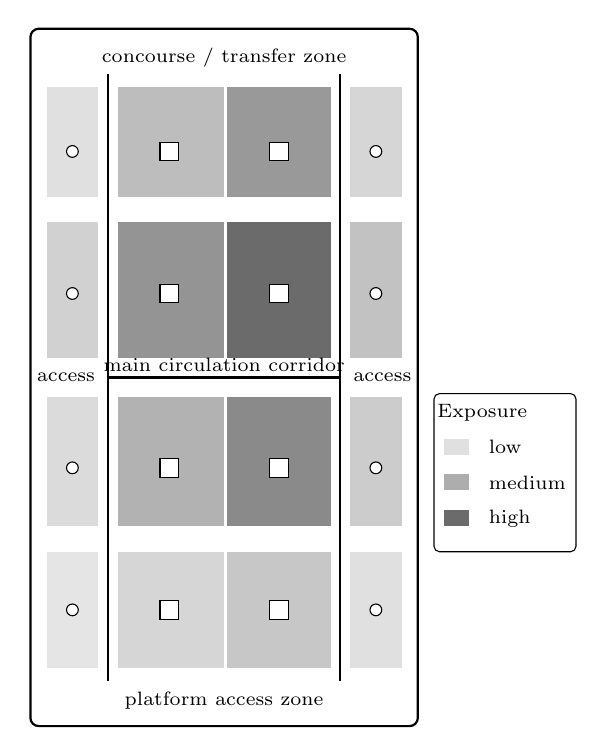
\begin{tikzpicture}[
    x=0.82cm,
    y=0.82cm,
    font=\small
]

% Outer boundary
\draw[rounded corners=3pt, thick] (0,0) rectangle (6,10.8);

% Main spatial structure
\draw[thick] (1.2,0.7) -- (1.2,10.1);
\draw[thick] (4.8,0.7) -- (4.8,10.1);
\draw[thick] (1.2,5.4) -- (4.8,5.4);

% Heatmap cells
\fill[black!10] (0.25,0.9) rectangle (1.05,2.7);
\fill[black!16] (1.35,0.9) rectangle (3.0,2.7);
\fill[black!22] (3.05,0.9) rectangle (4.65,2.7);
\fill[black!12] (4.95,0.9) rectangle (5.75,2.7);

\fill[black!14] (0.25,3.1) rectangle (1.05,5.1);
\fill[black!30] (1.35,3.1) rectangle (3.0,5.1);
\fill[black!46] (3.05,3.1) rectangle (4.65,5.1);
\fill[black!20] (4.95,3.1) rectangle (5.75,5.1);

\fill[black!18] (0.25,5.7) rectangle (1.05,7.8);
\fill[black!42] (1.35,5.7) rectangle (3.0,7.8);
\fill[black!58] (3.05,5.7) rectangle (4.65,7.8);
\fill[black!24] (4.95,5.7) rectangle (5.75,7.8);

\fill[black!12] (0.25,8.2) rectangle (1.05,9.9);
\fill[black!26] (1.35,8.2) rectangle (3.0,9.9);
\fill[black!40] (3.05,8.2) rectangle (4.65,9.9);
\fill[black!16] (4.95,8.2) rectangle (5.75,9.9);

% Devices
\foreach \x/\y in {0.65/1.8,0.65/4.0,0.65/6.7,0.65/8.9,5.35/1.8,5.35/4.0,5.35/6.7,5.35/8.9}
    \node[circle, draw, fill=white, inner sep=1.5pt] at (\x,\y) {};

\foreach \x/\y in {2.15/1.8,3.85/1.8,2.15/4.0,3.85/4.0,2.15/6.7,3.85/6.7,2.15/8.9,3.85/8.9}
    \node[rectangle, draw, fill=white, minimum width=0.14cm, minimum height=0.14cm] at (\x,\y) {};

% Labels
\node[font=\scriptsize] at (3,10.35) {concourse / transfer zone};
\node[font=\scriptsize] at (3,5.6) {main circulation corridor};
\node[font=\scriptsize] at (3,0.4) {platform access zone};
\node[font=\scriptsize] at (0.55,5.4) {access};
\node[font=\scriptsize] at (5.45,5.4) {access};

% Minimal legend
\draw[rounded corners=2pt] (6.25,2.7) rectangle (8.45,5.15);
\node[font=\scriptsize] at (7,4.85) {Exposure};

\fill[black!12] (6.4,4.2) rectangle (6.8,4.45);
\node[anchor=west, font=\scriptsize] at (6.95,4.32) {low};

\fill[black!32] (6.4,3.65) rectangle (6.8,3.9);
\node[anchor=west, font=\scriptsize] at (6.95,3.77) {medium};

\fill[black!58] (6.4,3.1) rectangle (6.8,3.35);
\node[anchor=west, font=\scriptsize] at (6.95,3.22) {high};

\end{tikzpicture}
% \fbox{%
% \parbox[c][6.0cm][c]{0.92\linewidth}{%
% \centering
% \textbf{Placeholder for TikZ figure}\\[0.5em]
% Conceptual station heatmap showing spatial variation in inferred maintenance exposure / cumulative proxy load across zones and device locations
% }}
\caption{Conceptual spatial heatmap of inferred maintenance exposure in the illustrative station setting. The figure should visualize how indirect operational information may be aggregated into zone-level or device-cluster-level maintenance relevance, highlighting areas of likely elevated burden rather than directly measured degradation.}
\label{fig:station-heatmap}
\end{figure}

In the context of the paper, the main value of such a heatmap is interpretive. It makes visible how LD-PdM can transform fragmented operational information into a planning-oriented representation of where maintenance attention is likely to matter most. It also provides a visual link between the abstract asymmetries discussed earlier and the practical logic of intervention prioritisation.

\subsection{From proxy-based inference to maintenance prioritisation}

A second important class of outputs concerns prioritisation rather than diagnosis. In the LD-PdM setting, the most useful result is often not a precise estimate of remaining useful life for every device, but a structured ranking of where inspections, preventive actions, or resource allocation should be focused first. This ranking may be defined at different levels of granularity: individual devices, device groups, functional zones, or station subsystems. The essential point is that the output supports action under uncertainty rather than claiming full observability.

In the illustrative station case, prioritisation can be understood as a mapping from inferred latent burden and associated uncertainty into maintenance attention classes. Devices or zones with higher inferred exposure, stronger contextual evidence of stress concentration, or more informative maintenance histories may be assigned higher inspection priority. Conversely, assets with lower inferred burden or more ambiguous relevance may be monitored less intensively or deferred when resources are limited. This kind of prioritisation is especially appropriate when maintenance teams must make decisions across many similar assets under limited time and staffing.

Importantly, prioritisation does not require all uncertainty to be resolved in advance. On the contrary, it is often valuable precisely because it allows weak but structured evidence to shape maintenance action before failures accumulate. The resulting decision logic is therefore ordinal rather than fully diagnostic: what matters is not whether the framework can certify the exact health state of a device, but whether it can support more plausible sequencing of maintenance effort than a baseline policy that ignores contextual evidence.

Figure~\ref{fig:priority-output} is intended as a simple visual placeholder for this type of output.

\begin{figure}[t]
\centering
% \fbox{%
% \parbox[c][4.8cm][c]{0.92\linewidth}{%
% \centering
% \textbf{Placeholder for TikZ figure}\\[0.5em]
% Illustrative prioritisation output, e.g. ranked zones / device groups, urgency classes, or risk bands derived from proxy-based inference
% }}
% ============================================================
% Figure: Illustrative prioritisation output
% ============================================================
\begin{tikzpicture}[
    x=0.9cm,
    y=0.78cm,
    font=\small,
    >=Latex
]

% Axes
\draw[->, thick] (0,0) -- (0,8.2) node[above] {Expected relevance};
\draw[->, thick] (0,0) -- (6.9,0) node[right] {Uncertainty};

% Threshold guides
\draw[dashed] (2.3,0) -- (2.3,8);
\draw[dashed] (4.6,0) -- (4.6,8);
\draw[dashed] (0,2.6) -- (6.6,2.6);
\draw[dashed] (0,5.3) -- (6.6,5.3);

% Region labels
\node[font=\scriptsize, align=center] at (1.15,7.9) {routine\\ planning};
\node[font=\scriptsize, align=center] at (3.45,7.9) {elevated\\ attention};
\node[font=\scriptsize, align=center] at (5.55,7.9) {inspect /\\ clarify};
\node[font=\scriptsize, align=center] at (1.15,1.2) {low priority};

% Points
\node[circle, draw, fill=white, inner sep=1.8pt] at (1.3,6.0) {};
\node[anchor=east, font=\scriptsize] at (1.15,6.0) {Z1};

\node[circle, draw, fill=white, inner sep=1.8pt] at (3.0,6.3) {};
\node[anchor=south, font=\scriptsize] at (3.0,6.45) {Z2};

\node[circle, draw, fill=white, inner sep=1.8pt] at (5.2,5.9) {};
\node[anchor=west, font=\scriptsize] at (5.35,5.9) {Z3};

\node[rectangle, draw, fill=white, minimum width=0.16cm, minimum height=0.16cm] at (1.7,4.2) {};
\node[anchor=west, font=\scriptsize] at (1.9,4.2) {E1};

\node[rectangle, draw, fill=white, minimum width=0.16cm, minimum height=0.16cm] at (3.8,4.6) {};
\node[anchor=west, font=\scriptsize] at (4.0,4.6) {E2};

\node[rectangle, draw, fill=white, minimum width=0.16cm, minimum height=0.16cm] at (5.3,4.0) {};
\node[anchor=west, font=\scriptsize] at (5.5,4.0) {E3};

\node[diamond, draw, fill=white, aspect=1.2, inner sep=1.3pt] at (1.5,1.7) {};
\node[anchor=west, font=\scriptsize] at (1.7,1.7) {D1};

\node[diamond, draw, fill=white, aspect=1.2, inner sep=1.3pt] at (2.9,2.0) {};
\node[anchor=west, font=\scriptsize] at (3.1,2.0) {D2};

\node[diamond, draw, fill=white, aspect=1.2, inner sep=1.3pt] at (4.9,1.5) {};
\node[anchor=west, font=\scriptsize] at (5.1,1.5) {D3};

% Callout
\draw[rounded corners=2pt] (6.3,7.25) rectangle (8.45,7.95);
\node[font=\scriptsize, align=center] at (7.38,7.6) {high relevance\\ high uncertainty};
\draw[->] (6.3,7.6) -- (5.2,6.05);

\end{tikzpicture}
\caption{Illustrative prioritisation output for the station-based LD-PdM case. The planned figure may take the form of ranked asset groups, zone-level urgency categories, or risk bands, with the purpose of showing how probabilistic beliefs are translated into maintenance action priorities rather than precise diagnosis.}
\label{fig:priority-output}
\end{figure}

The specific graphical form can be chosen later, but conceptually the figure should demonstrate that the framework produces actionable distinctions among assets or locations. This is the practical closure of the argument developed throughout the paper: limited and indirect information can still support maintenance decisions when it is treated as structured evidence about latent operational burden.

\subsection{Uncertainty-aware interpretation of maintenance signals}

A central feature of the LD-PdM perspective is that uncertainty is part of the output rather than an inconvenient residual. Two assets may have similar expected exposure while differing substantially in the confidence that can be attached to that estimate. One zone may appear important because of repeated proxy evidence from several sources, whereas another may appear risky primarily because of sparse but suggestive contextual indicators. A useful maintenance framework should preserve this distinction rather than collapsing all signals into a single unqualified score.

In practical terms, this means that maintenance-relevant outputs should be interpreted jointly in terms of expected burden and uncertainty. A device group with moderate inferred exposure but low uncertainty may justify routine scheduling, whereas a group with similar exposure but much higher uncertainty may justify exploratory inspection, additional data collection, or temporary elevation of maintenance attention until the uncertainty is reduced. In this sense, uncertainty is not only a measure of epistemic weakness, but also a guide for intervention strategy.

This interpretation is especially important in the present paper because it protects the framework from being misread as a hidden diagnostic model. The framework does not claim that proxy-based inference yields exact state estimates. Its value lies instead in its ability to make explicit what is known, what remains uncertain, and how those distinctions affect planning. In low-instrumentation environments, this transparency is often more useful than overconfident numerical precision.

A compact way to communicate this idea in the final version may be through a visual distinction between expected exposure and uncertainty band, or through a two-dimensional figure in which priority is influenced jointly by estimated burden and confidence. Such a figure is not strictly necessary, but the underlying conceptual point is important: in LD-PdM, uncertainty is itself maintenance-relevant information.

\subsection{What the illustrative case demonstrates and what remains outside scope}

The station-based example demonstrates that the LD-PdM framework can be instantiated in a concrete infrastructure setting using limited and indirect information. More specifically, it shows that maintenance reasoning can be organized around latent variables, proxy evidence, and explicit interpretive assumptions even when direct condition monitoring is weak or absent. It also shows that the outputs of such reasoning are naturally decision-oriented: spatial concentration of burden, prioritisation of inspections or interventions, and differentiated maintenance attention across zones or asset groups.

At the same time, the case is deliberately limited in scope. It is not intended as a full validation study, and it does not claim to provide exact degradation reconstruction, optimal maintenance scheduling, or deployment-ready prognostic performance. Likewise, the visualisations and probabilistic relationships introduced here are illustrative rather than final operational models. Their purpose is to make the inferential and decision-making logic of LD-PdM explicit, not to exhaust all technical details of station-scale simulation or maintenance optimisation.

This boundary is important both methodologically and strategically. Methodologically, it keeps the case aligned with the central contribution of the paper, which is conceptual and structural rather than algorithmic. Strategically, it preserves space for future work in which the station domain can be developed in greater technical depth, including richer simulation, calibration, validation, and comparative analysis. In the present manuscript, the case plays a different but still essential role: it shows that the asymmetries, probabilistic framing, and decision logic proposed in the preceding sections can be brought together into a coherent and practically interpretable LD-PdM workflow.

\section{Discussion}
\label{sec:discussion}

\subsection{What LD-PdM changes in how we evaluate ``success''}

A central implication of the LD-PdM framing is that conventional PdM evaluation criteria may be poorly aligned with operational value. In sensor-rich predictive maintenance, success is often expressed through fault-classification accuracy, remaining-useful-life error, or similar measures of predictive performance. Such metrics are appropriate when condition-relevant states are sufficiently observable and when failure histories are rich enough to support stable supervised inference. However, the argument developed in this paper is that these assumptions are systematically weakened in LD-PdM. When observability is limited and failure evidence is sparse, heterogeneous, or censored, the most useful outputs are often not deterministic predictions, but rankings, risk bands, and prioritisation policies that help allocate attention under uncertainty.

This shift changes what should count as a good model. In LD-PdM, success is better assessed in terms of decision-focused criteria such as reduction in unplanned downtime, improved utilisation of maintenance crews and spare parts, stability of prioritisation under uncertain evidence, and transparency of the assumptions that connect proxy information to action. This view is consistent with the broader risk-based maintenance perspective represented by \citet{Yeter2020}, who formulate maintenance planning in terms of risk and lifecycle consequences rather than prediction alone. It is also consistent with the Bayesian decision-support logic reviewed by \citet{Kabir2019154}, where the value of a model lies not only in inferential power, but in its ability to structure uncertain evidence in a way that supports action. At a more general level, \citet{Straub2015} provide the conceptual basis for this shift by treating engineering analysis as belief updating in service of decision-making rather than as mere state estimation.

In practical terms, this suggests that LD-PdM studies may be evaluated through criteria such as the stability of maintenance rankings under uncertainty, the reduction of reactive interventions, the quality of inspection allocation, and the sensitivity of decisions to proxy-data assumptions. Such criteria do not replace quantitative assessment; they redirect it toward the operational consequences of acting under weak evidence. The relevant question is often not whether a model recovers the latent ``true'' health state of an asset with high precision, but whether it supports robust and useful decisions despite limited observability. In that sense, LD-PdM extends the logic of risk-based maintenance into a data-constrained regime where uncertainty is not eliminated, but managed explicitly.

\subsection{Relation to existing maintenance paradigms}

A broader implication of the LD-PdM framing is that data scarcity should not be treated merely as a technical inconvenience within conventional PdM, but as a defining property of a distinct maintenance regime with its own modelling assumptions, evidential limits, and decision criteria. This point becomes clearer when LD-PdM is positioned relative to existing maintenance paradigms. Classical condition-based maintenance assumes that at least some meaningful condition information is directly available for monitoring and intervention. Mainstream data-driven PdM extends this idea by coupling condition information with statistical or machine-learning models, often under assumptions of sufficient historical data, identifiable fault signatures, and trainable predictive relationships \citep{Selcuk20171670,Carvalho2019,Cinar2020}. By contrast, risk-based maintenance contributes a different emphasis: consequences, uncertainty, and the value of action matter as much as prediction itself \citep{Yeter2020,Straub2015}.

LD-PdM occupies an intermediate but distinct position among these paradigms. It shares with risk-based maintenance an emphasis on uncertainty, consequences, and decision support, but it also shares with contemporary PdM an interest in structured evidence integration and operational prediction. Its distinguishing feature is that it treats limited observability as a structural property of the maintenance setting rather than as a temporary modelling deficiency. In this sense, LD-PdM should not be interpreted as a failed approximation of sensor-rich PdM, but as a regime in which the evidential basis of maintenance reasoning is fundamentally different.

This positioning is important because it changes how the contribution of the paper should be read. The present work does not propose a new diagnostic algorithm, nor does it argue that proxy-based reasoning is universally preferable to direct condition monitoring. Rather, it identifies a class of maintenance problems for which conventional data-centric assumptions are systematically misaligned with the economic and informational realities of the system. Recognising this regime explicitly helps explain why low-observability maintenance problems require different modelling expectations, different forms of validation, and different notions of practical success.

\subsection{Relation to sensor-rich PdM and digital twin narratives}

The LD-PdM perspective is not intended as a rejection of sensor-rich predictive maintenance or of digital twin approaches. Rather, it clarifies that these approaches address only part of the broader maintenance landscape. As reviewed by \citet{vanDinter2022}, much of the digital-twin-for-maintenance literature assumes comparatively rich data environments in which operational, condition, and model information can be integrated into detailed virtual representations. Similarly, \citet{Yu2021} demonstrate how digital-twin-based decision frameworks can support operation and maintenance in infrastructure contexts when the digital representation is sufficiently informative. These contributions are important, but they also illustrate the extent to which current digital twin narratives often presuppose a level of observability that is not universally available.

LD-PdM highlights a complementary possibility. Even in the absence of dense condition-monitoring streams, digital representations may still create maintenance value by serving as integration layers for proxy information, contextual variables, maintenance history, and explicit assumptions about dependence structure. In such settings, the twin is useful not because it provides complete observability, but because it helps organize heterogeneous evidence, expose uncertainty, and support decision workflows. This interpretation is compatible with the data-integration logic discussed by \citet{Ma2020}, who show that maintenance decision support in facility-oriented contexts may depend on combining multiple information sources rather than relying exclusively on direct health measurements.

This distinction matters for positioning. LD-PdM does not compete with sensor-rich PdM by claiming that proxy-based reasoning is universally superior. Instead, it addresses contexts in which sensor-rich approaches are systematically economically disfavoured, organizationally unrealistic, or technically unavailable. The contribution of the present paper is therefore not a new digital twin platform, nor a new prognostic algorithm, but a framework for reasoning about maintenance under structural asymmetry. This helps avoid over-promising while also making clear that low-observability maintenance should not be treated as a pathological exception outside the scope of PdM.

\subsection{Methodological implications and open research directions}

The LD-PdM framing brings into focus several methodological directions that are easy to overlook when PdM is defined primarily through direct sensing and supervised prediction. First, it strengthens the case for models that combine heterogeneous proxy evidence with explicit prior assumptions. In data-rich settings, priors can be treated as optional modelling choices; in LD-PdM, they are often structurally necessary because the evidence is too weak to support inference on its own. This reinforces the role of transparent probabilistic models, especially when expert knowledge and incomplete observations must be combined in an auditable way, as emphasized by \citet{Baraldi2015176} and \citet{Kabir2019154}.

Second, LD-PdM foregrounds the need for honest treatment of censoring, interrupted trajectories, and rare events. The relevance of such issues is well illustrated by \citet{Zeng2016253}, who discuss inference under interval-censored data, and by \citet{Bourinet2016210}, who address rare-event estimation in reliability settings where evidence is scarce and conventional sampling logic becomes fragile. These are not peripheral technical details. In many low-instrumentation maintenance environments, they are part of the basic structure of the problem. As a result, future work in LD-PdM should place greater emphasis on modelling frameworks that preserve these uncertainties rather than smoothing them away to fit standard machine-learning workflows.

A further methodological implication is that LD-PdM still lacks a well-developed canon of proxy-based inference methods tailored specifically to maintenance planning in low-instrumentation environments. For this reason, progress may depend partly on adapting ideas from indirect measurement and state-reconstruction problems in other engineering domains, while translating them into maintenance-relevant forms of uncertainty representation, prioritisation, and decision support. Studies such as those by \citet{Sun20248912}, \citet{Zhou2025}, and \citet{Guo2025} show how practically relevant quantities may be inferred from secondary, indirect, or context-dependent observations through explicit models of dependence. Although these works do not concern maintenance planning directly, they share an epistemic structure that is highly relevant to LD-PdM: the object of interest is latent, the evidence is partial, and inference depends on structured assumptions rather than direct observation. This suggests that progress in LD-PdM may come not only from new algorithms, but also from better representations of indirect evidence, clearer problem formulations, and evaluation protocols that match the regime being studied.

Finally, LD-PdM points toward the importance of human-interpretable uncertainty communication. If maintenance planners are expected to act on weak and indirect evidence, then the representation of assumptions, uncertainty bands, and prioritisation logic becomes part of the method itself rather than a secondary reporting issue. In this respect, the methodological challenge is as much about making inference communicable as it is about making it computationally tractable.

\subsection{Threats to validity and boundary conditions}

The argument developed in this paper has clear boundary conditions. LD-PdM is not intended as a universal predictive-maintenance paradigm, but as a regime that becomes relevant under a specific combination of observability, cost structure, and operational value. If failures are extremely rare and their consequences negligible, even a risk-based prioritisation model may not justify the effort of building and maintaining an inference framework. At the opposite extreme, if assets are strongly safety-critical and the consequences of failure are severe, the case for additional instrumentation may become economically justified, shifting the problem back toward sensor-rich PdM. In this sense, LD-PdM is most relevant in an intermediate zone: systems with high aggregate impact across populations, meaningful downtime or service costs, but weak incentives to instrument each unit individually.

A second threat concerns confounding and instability in proxy-based inference. Contextual variables may correlate with usage without causally driving degradation, and relationships that appear stable under one operational regime may break when traffic patterns, maintenance practices, or system usage change. This is one reason why the probabilistic and explicit-assumption perspective advanced in this paper is important. As argued by \citet{Straub2015}, uncertainty should be treated as an explicit part of engineering reasoning, not as residual noise. Likewise, the Bayesian reliability perspective reviewed by \citet{Kabir2019154} suggests that such uncertainty is best managed through models that expose assumptions rather than conceal them. Under LD-PdM conditions, conservative modelling and incremental updating are therefore preferable to brittle point predictions built on implicitly fixed proxy relationships.

A third boundary concerns the role of digital and virtual sensing. Work such as \citet{Mahmoodian2022} shows that digital twins and intelligent maintenance infrastructures can create substantial value in civil and infrastructure applications, but such approaches may also depend on a richer information environment than is available in many mass-deployed systems. This reinforces an important point: LD-PdM is not an argument against better sensing, but a framework for situations in which better sensing is not presently justified or available. Its validity therefore depends on honesty about what remains latent, what evidence is genuinely available, and how far proxy-based reasoning can be trusted before the case for additional instrumentation should be reconsidered.

Taken together, these limitations do not undermine the LD-PdM concept; rather, they help define its appropriate scope. The value of the framework lies precisely in making these constraints explicit, so that predictive maintenance in low-observability settings can be discussed as a legitimate engineering problem with identifiable assumptions, limits, and decision consequences.
% ============================================================
\section{Conclusions}
\label{sec:conclusions}

Predictive maintenance is often described as a sensor-driven path to accurate diagnosis and prognostics. This paper has argued that a large class of real systems does not fit that picture. In many economically relevant maintenance settings, needs may be substantial while condition-monitoring data remain structurally scarce, indirect, or entirely absent due to cost, legacy infrastructure, or organisational constraints. We refer to this regime as \emph{Limited-Data Predictive Maintenance} (LD-PdM) and argue that it should be treated not as a failed approximation of sensor-rich PdM, but as a distinct maintenance regime with its own evidential structure, modelling assumptions, and criteria of success.

The main contribution of the paper is therefore conceptual and structural rather than algorithmic. We have shown that LD-PdM can be framed coherently as inference and decision support under uncertainty, organized around four asymmetries: limited observability of decision-relevant states, sparse and biased failure evidence, economic constraints on instrumentation, and the mismatch between weak asset-level observability and meaningful population-level decision value. Under these conditions, predictive maintenance remains possible, but its outputs should be understood differently. The relevant targets are often prioritisation, scheduling, risk bands, and resource allocation policies rather than deterministic per-asset diagnosis or highly resolved remaining-useful-life estimates.

A second conclusion is methodological. In low-instrumentation settings, useful maintenance reasoning depends on the explicit integration of proxy evidence, prior knowledge, maintenance history, and uncertainty representation. This shifts attention from purely sensor-centric modelling toward transparent belief updating and decision-oriented interpretation. The illustrative station-based case was included in this paper to show that such a perspective is operationally meaningful even when direct degradation measurements are unavailable. A more technical implementation of the same general logic, focused on railway-station doors and elevators and using Bayesian proxy-flow modelling with scheduling integration, is developed in the companion conference paper \citep{GPECOM2026LdPDM}.

The broader practical message is not that sensors are unnecessary, but that the absence of rich sensing should not automatically exclude a system from predictive-maintenance reasoning. In many cases, ``lack of sensors'' is better understood as a design constraint than as a reason to retreat to purely reactive or calendar-based maintenance. LD-PdM therefore reframes predictive maintenance for a wide class of mass-deployed infrastructure and service assets whose operating burden can be inferred only indirectly. Future work should focus on evaluation protocols aligned with decision outcomes, stronger methods for proxy-based inference under censoring and rare events, and tighter integration of low-data maintenance reasoning with operational planning and digital representations of infrastructure systems.



\vspace{6pt} 

%%%%%%%%%%%%%%%%%%%%%%%%%%%%%%%%%%%%%%%%%%
%% optional
%\supplementary{The following supporting information can be downloaded at:  \linksupplementary{s1}, Figure S1: title; Table S1: title; Video S1: title.}

% Only for journal Methods and Protocols:
% If you wish to submit a video article, please do so with any other supplementary material.
% \supplementary{The following supporting information can be downloaded at: \linksupplementary{s1}, Figure S1: title; Table S1: title; Video S1: title. A supporting video article is available at doi: link.}

% Only used for preprtints:
% \supplementary{The following supporting information can be downloaded at the website of this paper posted on \href{https://www.preprints.org/}{Preprints.org}.}

% Only for journal Hardware:
% If you wish to submit a video article, please do so with any other supplementary material.
% \supplementary{The following supporting information can be downloaded at: \linksupplementary{s1}, Figure S1: title; Table S1: title; Video S1: title.\vspace{6pt}\\
%\begin{tabularx}{\textwidth}{lll}
%\toprule
%\textbf{Name} & \textbf{Type} & \textbf{Description} \\
%\midrule
%S1 & Python script (.py) & Script of python source code used in XX \\
%S2 & Text (.txt) & Script of modelling code used to make Figure X \\
%S3 & Text (.txt) & Raw data from experiment X \\
%S4 & Video (.mp4) & Video demonstrating the hardware in use \\
%... & ... & ... \\
%\bottomrule
%\end{tabularx}
%}

%%%%%%%%%%%%%%%%%%%%%%%%%%%%%%%%%%%%%%%%%%
% \authorcontributions{For research articles with several authors, a short paragraph specifying their individual contributions must be provided. The following statements should be used ``Conceptualization, X.X. and Y.Y.; methodology, X.X.; software, X.X.; validation, X.X., Y.Y. and Z.Z.; formal analysis, X.X.; investigation, X.X.; resources, X.X.; data curation, X.X.; writing--original draft preparation, X.X.; writing--review and editing, X.X.; visualization, X.X.; supervision, X.X.; project administration, X.X.; funding acquisition, Y.Y. All authors have read and agreed to the published version of the manuscript.'', please turn to the  \href{http://img.mdpi.org/data/contributor-role-instruction.pdf}{CRediT taxonomy} for the term explanation. Authorship must be limited to those who have contributed substantially to the work~reported.}

\funding{Partially Funded by the European Union. Views and opinion expressed are however those of the author(s) only and do not necessarily reflect those of the European Union or Europe’s Rail Joint Undertaking. Neither the European Union nor the granting authority can be held responsible for them. The project FP3-IAM4Rail is supported by the Europe's Rail Joint Undertaking and its members. 
Partially funded by AGH's Subvention for scientific research.}

\institutionalreview{Not applicable}

\informedconsent{Not applicable}

\dataavailability{No new data were created.} 

%\durcstatement{Current research is limited to the [please insert a specific academic field, e.g., XXX], which is beneficial [share benefits and/or primary use] and does not pose a threat to public health or national security. Authors acknowledge the dual-use potential of the research involving xxx and confirm that all necessary precautions have been taken to prevent potential misuse. As an ethical responsibility, authors strictly adhere to relevant national and international laws about DURC. Authors advocate for responsible deployment, ethical considerations, regulatory compliance, and transparent reporting to mitigate misuse risks and foster beneficial outcomes.}

% Only for journal Nursing Reports
%\publicinvolvement{Please describe how the public (patients, consumers, carers) were involved in the research. Consider reporting against the GRIPP2 (Guidance for Reporting Involvement of Patients and the Public) checklist. If the public were not involved in any aspect of the research add: ``No public involvement in any aspect of this research''.}
%
%% Only for journal Nursing Reports
%\guidelinesstandards{Please add a statement indicating which reporting guideline was used when drafting the report. For example, ``This manuscript was drafted against the XXX (the full name of reporting guidelines and citation) for XXX (type of research) research''. A complete list of reporting guidelines can be accessed via the equator network: \url{https://www.equator-network.org/}.}
%
%% Only for journal Nursing Reports
%\useofartificialintelligence{Please describe in detail any and all uses of artificial intelligence (AI) or AI-assisted tools used in the preparation of the manuscript. This may include, but is not limited to, language translation, language editing and grammar, or generating text. Alternatively, please state that “AI or AI-assisted tools were not used in drafting any aspect of this manuscript”.}

\acknowledgments{During the preparation of this manuscript the author used Chat GPT 5.4 for the purposes of stylistic corrections. The author has reviewed and edited the output and take full responsibility for the content of this publication.}

\conflictsofinterest{The author declare no conflicts of interest.} 

%%%%%%%%%%%%%%%%%%%%%%%%%%%%%%%%%%%%%%%%%%
%% Optional

%% Only for journal Encyclopedia
%\entrylink{The Link to this entry published on the encyclopedia platform.}

\abbreviations{Abbreviations}{
The following abbreviations are used in this manuscript:
\\

\noindent 
\begin{tabular}{@{}ll}
PdM & Predictive maintenance\\
LD-PdM & Limited-Data Predictive Maintenance\\
RUL & Remaining useful life
\end{tabular}
}

% %%%%%%%%%%%%%%%%%%%%%%%%%%%%%%%%%%%%%%%%%%
% %% Optional
% \appendixtitles{no} % Leave argument "no" if all appendix headings stay EMPTY (then no dot is printed after "Appendix A"). If the appendix sections contain a heading then change the argument to "yes".
% \appendixstart
% \appendix
% \section[\appendixname~\thesection]{}
% \subsection[\appendixname~\thesubsection]{}
% The appendix is an optional section that can contain details and data supplemental to the main text--for example, explanations of experimental details that would disrupt the flow of the main text but nonetheless remain crucial to understanding and reproducing the research shown; figures of replicates for experiments of which representative data are shown in the main text can be added here if brief, or as Supplementary Data. Mathematical proofs of results not central to the paper can be added as an appendix.

% \begin{table}[H] 
% \caption{This is a table caption.\label{tab5}}
% %\newcolumntype{C}{>{\centering\arraybackslash}X}
% \begin{tabularx}{\textwidth}{CCC}
% \toprule
% \textbf{Title 1}	& \textbf{Title 2}	& \textbf{Title 3}\\
% \midrule
% Entry 1		& Data			& Data\\
% Entry 2		& Data			& Data\\
% \bottomrule
% \end{tabularx}
% \end{table}

% \section[\appendixname~\thesection]{}
% All appendix sections must be cited in the main text. In the appendices, Figures, Tables, etc. should be labeled, starting with ``A''--e.g., Figure A1, Figure A2, etc.

%%%%%%%%%%%%%%%%%%%%%%%%%%%%%%%%%%%%%%%%%%
%\isPreprints{}{% This command is only used for ``preprints''.
\begin{adjustwidth}{-\extralength}{0cm}
%} % If the paper is ``preprints'', please uncomment this parenthesis.
%\printendnotes[custom] % Un-comment to print a list of endnotes

\reftitle{References}

% Please provide either the correct journal abbreviation (e.g. according to the “List of Title Word Abbreviations” http://www.issn.org/services/online-services/access-to-the-ltwa/) or the full name of the journal.
% Citations and References in Supplementary files are permitted provided that they also appear in the reference list here. 

%=====================================
% References, variant A: external bibliography
%=====================================

\bibliography{extracted} % <-- set your .bib filename here



%=====================================
% References, variant B: internal bibliography
%=====================================




% If authors have biography, please use the format below
%\section*{Short Biography of Authors}
%\bio
%{\raisebox{-0.35cm}{\includegraphics[width=3.5cm,height=5.3cm,clip,keepaspectratio]{Definitions/author1.pdf}}}
%{\textbf{Firstname Lastname} Biography of first author}
%
%\bio
%{\raisebox{-0.35cm}{\includegraphics[width=3.5cm,height=5.3cm,clip,keepaspectratio]{Definitions/author2.jpg}}}
%{\textbf{Firstname Lastname} Biography of second author}

% For the MDPI journals use author-date citation, please follow the formatting guidelines on http://www.mdpi.com/authors/references
% To cite two works by the same author: \citeauthor{ref-journal-1a} (\citeyear{ref-journal-1a}, \citeyear{ref-journal-1b}). This produces: Whittaker (1967, 1975)
% To cite two works by the same author with specific pages: \citeauthor{ref-journal-3a} (\citeyear{ref-journal-3a}, p. 328; \citeyear{ref-journal-3b}, p.475). This produces: Wong (1999, p. 328; 2000, p. 475)

%%%%%%%%%%%%%%%%%%%%%%%%%%%%%%%%%%%%%%%%%%
%% for journal Sci
%\reviewreports{\\
%Reviewer 1 comments and authors’ response\\
%Reviewer 2 comments and authors’ response\\
%Reviewer 3 comments and authors’ response
%}
%%%%%%%%%%%%%%%%%%%%%%%%%%%%%%%%%%%%%%%%%%
\PublishersNote{}
%\isPreprints{}{% This command is only used for ``preprints''.
\end{adjustwidth}
%} % If the paper is ``preprints'', please uncomment this parenthesis.
\end{document}

